\documentclass[10pt,oneside]{memoir}
\usepackage{layouts}[2001/04/29]
\makeglossary
\makeindex

\def\mychapterstyle{default}
\def\mypagestyle{headings}
\def\revision{}

%%% need more space for ToC page numbers
\setpnumwidth{2.55em}
\setrmarg{3.55em}

%%% need more space for ToC section numbers
\cftsetindents{part}{0em}{3em}
\cftsetindents{chapter}{0em}{3em}
\cftsetindents{section}{3em}{3em}
\cftsetindents{subsection}{4.5em}{3.9em}
\cftsetindents{subsubsection}{8.4em}{4.8em}
\cftsetindents{paragraph}{10.7em}{5.7em}
\cftsetindents{subparagraph}{12.7em}{6.7em}

%%% need more space for LoF numbers
\cftsetindents{figure}{0em}{3.0em}

%%% and do the same for the LoT
\cftsetindents{table}{0em}{3.0em}

%%% set up the page layout
\settrimmedsize{\stockheight}{\stockwidth}{*}	% Use entire page
\settrims{0pt}{0pt}

\setlrmarginsandblock{1.5in}{1.5in}{*}
\setulmarginsandblock{1.5in}{1.5in}{*}

\setmarginnotes{17pt}{51pt}{\onelineskip}
\setheadfoot{\onelineskip}{2\onelineskip}
\setheaderspaces{*}{2\onelineskip}{*}
\checkandfixthelayout

\usepackage{fontspec}
\setromanfont[Mapping=tex-text]{Palatino}

\usepackage{fancyvrb}			% Allow \verbatim et al. in footnotes
\usepackage{graphicx}			% To include graphics in pdf's (jpg, gif, png, etc)
\usepackage{booktabs}			% Better tables
\usepackage{tabulary}			% Support longer table cells
%\usepackage[utf8]{inputenc}		% For UTF-8 support

% \usepackage[T1]{fontenc}		% Use T1 font encoding for accented characters
\usepackage{xcolor}				% Allow for color (annotations)
% diagonal top left cell in tables
\usepackage{slashbox}
% for tables in the appendix
\usepackage[section]{placeins}
\usepackage{geometry}


%\geometry{landscape}			% Activate for rotated page geometry

%\usepackage[parfill]{parskip}	% Activate to begin paragraphs with an empty
								% line rather than an indent


\def\myauthor{Author}			% In case these were not included in metadata
\def\mytitle{Title}
\def\mykeywords{}
\def\mybibliostyle{plain}
\def\bibliocommand{}

\VerbatimFootnotes
\def\myauthor{Alexy Khrabrov}
\def\baseheaderlevel{2}
\def\format{complete}
\def\latexxslt{memoir-thesis-xelatex.xslt}
\def\mytitle{The Mind Economy of Social Networks: Dynamic Graph Analysis of Communications}


%
%	PDF Stuff
%

%\ifpdf							% Removed for XeLaTeX compatibility
%  \pdfoutput=1					% Removed for XeLaTeX compatibility
  \usepackage[
  	plainpages=false,
  	pdfpagelabels,
  	pdftitle={\mytitle},
  	pagebackref,
  	pdfauthor={\myauthor},
  	pdfkeywords={\mykeywords}
  	]{hyperref}
  \usepackage{memhfixc}
%\fi							% Removed for XeLaTeX compatibility


%
% Title Information
%


\ifx\latexauthor\undefined
\else
	\def\myauthor{\latexauthor}
\fi

\ifx\subtitle\undefined
\else
	\addtodef{\mytitle}{}{ \\ \subtitle}
\fi

\ifx\affiliation\undefined
\else
	\addtodef{\myauthor}{}{ \\ \affiliation}
\fi

\ifx\address\undefined
\else
	\addtodef{\myauthor}{}{ \\ \address}
\fi

\ifx\phone\undefined
\else
	\addtodef{\myauthor}{}{ \\ \phone}
\fi

\ifx\email\undefined
\else
	\addtodef{\myauthor}{}{ \\ \email}
\fi

\ifx\web\undefined
	\else
		\addtodef{\myauthor}{}{ \\ \web}
\fi

\title{\mytitle}
\author{\myauthor}

\begin{document}

\chapterstyle{\mychapterstyle}
\pagestyle{\mypagestyle}

%
%		Front Matter
%

\frontmatter


% Title Page

\maketitle
\clearpage

% Copyright Page
\vspace*{\fill}

\setlength{\parindent}{0pt}

\ifx\mycopyright\undefined
\else
	\textcopyright{} \mycopyright
\fi

\revision

\begin{center}
\framebox{ \parbox[t]{1.5in}{\centering Formatted for \LaTeX  \\ 
 by MultiMarkdown}}
\end{center}

\setlength{\parindent}{1em}
\clearpage

%
% Main Content
%


% Layout settings
\setlength{\parindent}{1em}

\mainmatter
\chapter{Success is Earned}
\label{successisearned}

\section{Abstract}
\label{abstract}

In their 1955 seminal book ``Personal Influence,'' Katz and Lazarsfeld \cite{katz1955influence} proposed the concept of influentials in social networks, propagating and filtering media streams in their communities.  Watts and Dodds, in their own 2008 paper, popularly known as ``Accidental Influentials,'' had shown that for a diffusion model with cascades, it's not necessary to have influentials to excite a typical network.  A Twitter study co-authored by Watts shows that influentials are not propagating URLs much better than the rest of us.  So are these influentials indeed accidental?


We look at a basic form of influence, showing how effective a communicator a person is in the social network.  We use our own reciprocal social capital as a metric keeping track how a person prioritizes his or her replies, paying attention to ``communication balances'' owed and to whom -- e.g., answering questions of somebody with a high social capital more often.  Any such metric induces a ranking among the users, and we build a class system on top of this ranking, resembling a human hierarchy of wealth.


In order to see whether the influence hierarchy is random or not, we simulate many parallel worlds, where users talk to each other based on various global and local optimization criteria.  Some of these criteria are simple, such as attaching randomly, or proportionally to the global in-degrees; some are complex, such as attach to a friend of a friend proportionally to their own mentions or social capital; or, ultimately, optimize your local capital gain locally, using the same reward function which is the foundation of the final ranking.  We either simulate the new worlds from scratch, or seed them with a few weeks of the real dynamic graph.  In all cases, we preserve the order of users joining the network and their out-degrees for each day.


Having built the dynamic hierarchy of influencers, changing daily within its own world, we compare the winners in the corresponding positions with the real ones, and across the worlds.  We look at the staying power in the same class bucket across days within the same world, and overlap of the respective buckets across different instances of the same world type, seeded with different lengths of reality to obtain week-shifted ones, or across different worlds altogether.


We observe that the more intelligent a simulation is, the higher is its staying power, showing that the influencers -- those in the higher classes -- are not random in their own worlds.  The overlap of the simulated influencers with the real-world ones is minimal, but also increases with more intelligent attachment strategies.


Our conclusions are as follows.


\begin{itemize}


\item the influentials are not random in their own worlds -- they correspond best to what the attachment strategies are the common rules in these worlds, but they are also those nodes who were well-positioned in their network to take advantage of these rules.  For instance, a global uniform attachment leads to the same stable celebrity bucket (the top one), even though the rest are churning through.  These celebrities stay very stable during the lifespan of their world, but are totally different across various runs of the uniform world.  At the same time, top buckets of smarter simulations show overlaps higher than 50\%, more than overlap of any other two simulations, showing that their success under the rules of those worlds is repeatable even when many edges are rearranged, and thus is not random.




\item the overlap with the real winners is small, proving that the winners in this world are lucky to have the set of rules which distinguished them.  If the accepted attachment strategies were slightly different, others would easily replace the current winners in some of the top buckets, and stay there under wide ranges of new conditions and their combinations.  In that sense, if we agree that our world with its own communication rules is itself random in a series of many similar ones where such rules can be slightly altered, the influencers might indeed be accidental. 




\item simply prescribing a desirable distribution of influence from the real world, as we do with {\itshape creps} simulations, leads to a stable and reproducible middle class.  It shows that order leads to a stable economy.




\item the middle and upper middle classes of social networks is less random across the more intelligent simulations, and is the main discovery of this thesis.  They carry 40\% of all communications, while comprising (roughly) only 20-25\% of population.  These users are the actual majority influencers, and they got where they are due to a diligent attention to communication, its priorities, dynamics, and energy demands.  In that sense, we conclude that success is earned.




\item mixed strategies optimizing communication efficiency can achieve staying power rates higher than in real world -- which means that the real world is not optimal in a sense, and reciprocal social capital, with its underlying communication balance, is not the only criteria used by real people, of course.  However, increasing capital efficiency, we capture more of the real winners, in several cases near 10\%, proving that it is in fact consistent with the behavior of many successful communicators on Twitter.



\end{itemize}

Figure~\ref{figure:heatmap-srates-medians-3wk} shows how several groups of simulations, loosely corresponding to either Katz-Lazarsfeld or Watts-Dodds models, relate to reality and each other.  Or social-capital based models, taking into account many feature of influencers as effective communicators, end up close to each other and reality, as compared to many simpler simulations, based on either uniform, or mentions-based attachment, such as the simulations of Watts-Dodds.



\begin{figure}
\begin{center}
    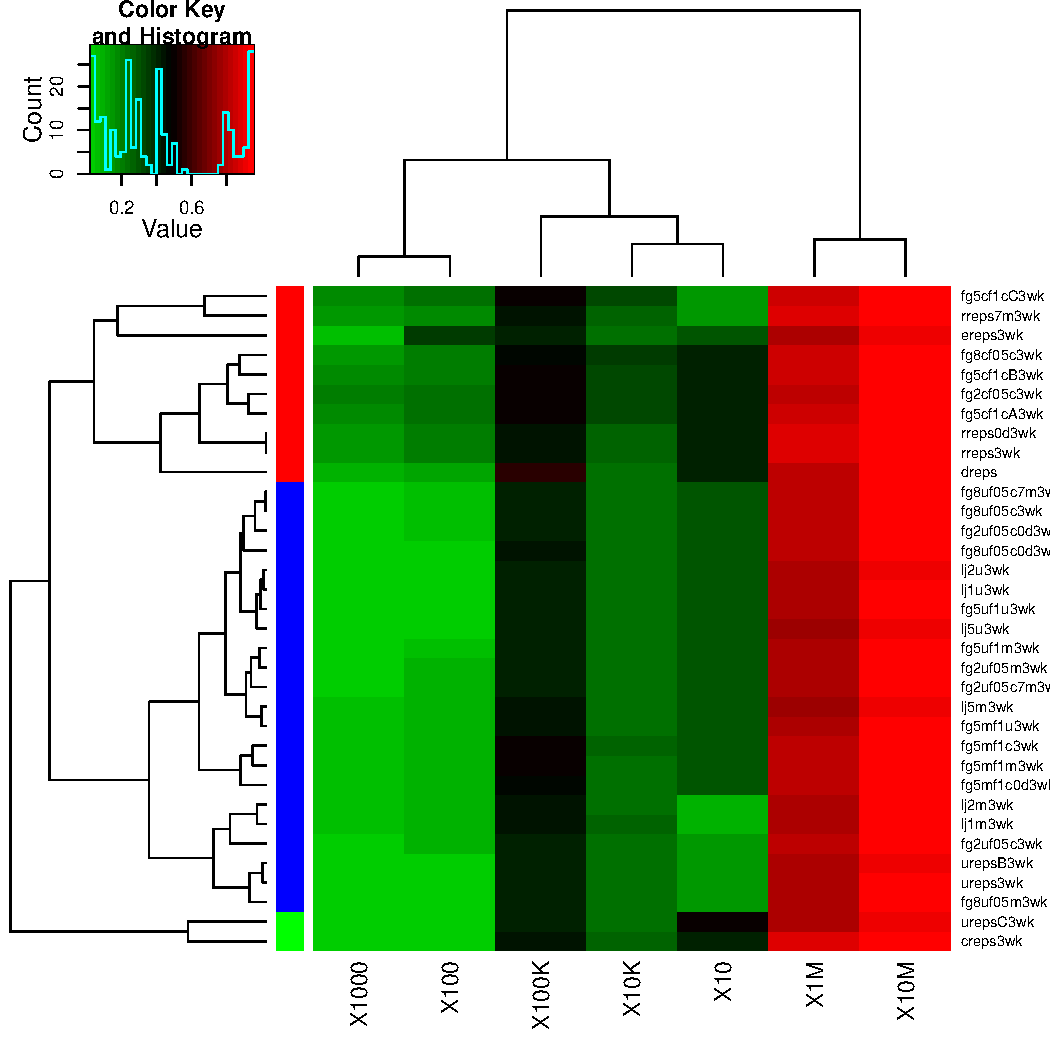
\includegraphics{figures/heatmap-srates-medians-3wk}
    \caption{Clustering of all simulations seeded by 3 weeks of reality, by staying power.  \emph{Dreps}, the reality, ends up together with our most intelligent capital-based worlds (red), reflecting Katz-Lazarsfeld better,  while uniform or mentions-based worlds (blue), similar to Watts-Dodds simulations, end up in a more distant cluster.}
    \label{figure:heatmap-srates-medians-3wk}
\end{center}
\end{figure}
\pagebreak \section{Accidental Influentials, or Not?}
\label{accidentalinfluentialsornot}

In the 1955 seminal book ``Personal Influence,'' Katz and Lazarsfeld proposed the concept of influentials in social networks, propagating and filtering media streams in their communities.  Although the focus of their study was information diffusion, Katz and Lazarsfeld for the first time fused media studies with dynamics of social groups at local level, and they identified many features of their opinion leaders which position those influentials as important community members by many criteria.


Watts and Dodds, in their 2008 paper, popularly known as ``Accidental Influentials,'' had shown that for a diffusion model with cascades, it's not necessary to have influentials to excite a typical network -- it's mostly the average low threshold on excitability of a majority which decides whether a full cascade will occur or not, instead of who started it, an influential or not.  Despite the specific setting, the idea that influentials are somehow ``accidental'' took a life of its own, and was reported by Harvard Business Review as one of Watts' key contributions for a list of the influential innovators for the next decade (presumably not accidental).


Since we study influence in real social networks, we took this question as a starting point, and for our family of metrics, ask: are our influentials accidental, or not?  And what can this question possibly mean, for a broad class of definitions of influence, which are many?


Let's say that we pick some definition of influence which suits a problem at hand.  The only general requirement for an influence measure we impose is that it establishes an order, or ranking, among all of the people in the study; and that the ``top influentials'' are simply the most highly ranked people in this list.  A consideration of influence then can focus on the very top, or look broadly at the classes of influence, similarly to the rich, the poor, and the middle class in a human economy.


Then our question can be made more concrete as follows: if influence is a function of behavior and connectivity, can we generally say that somebody becomes influential due to their ``intrinsic'' qualities, such as efficient behavior, or, on the contrary, is their influence mostly a product of luck, such as the propitious time and place of that individual's appearance in the network?


\section{Taught by Randomness}
\label{taughtbyrandomness}

The way to answer a philosophical question about whether something is random in this world or not is to create parallel worlds with slightly different rules, mix them with the real one at some point, and see what happens in the same way --- or differently.  When creating the new worlds by varying one feature at a time, we can hope to tease apart the features which make a difference in the course of events.  In this world, there's only one Twitter, albeit its character is constantly changing.  For any given dataset, we have only one order of influentials for any one metric.  However, we can separate the components of behavior which contribute to that influence, and, preserving some part of the network position and some of the behavior, alter the other parts, to see how the influence is affected.  By teasing the starting conditions and the behaviors apart, we can hope to get to the root of our main question.


We introduce a series of strategies to grow the graph from some point onwards, using a combination of behaviors which we reward in the actual graph, as the rewards in the random ones.  First of all, we keep the dynamic characteristics of all simulations the same in the following sense:


\begin{itemize}


\item we add the same new users on the same days as in the original graph

\item every user has the same outdegree for each day as in the original graph
\end{itemize}

Thus, we only rearrange the sinks of some edges in the simulation, after a certain point in time.  We use three classes of strategies to attach the edges:


\begin{itemize}


\item local utility -- optimizing exactly the same reward used to compute the social capital used to rank influence in the first place, but only for the action under control of a node, i.e.\ to whom it will reply (not from whom it will get the replies).  The latter would be a global optimization, while the former is still an individual one.

\item local friends-of-friends -- this strategy attaches to a friend of a friend with attractive characteristics, e.g.\ likely to be seen due to a large number of his/her own friends, mentions, or their own reciprocal social capital.

\item global -- this strategy approximates following users notable via global phenomena, such as celebrities or trendy ones, or efficient communicators with overall leading social capital rank.
\end{itemize}

In each simulated world, we mix these strategies via jump probabilities, creating a composite behavior, hopefully capturing some subset of the real world.  We see who wins in the simulated world, and compare the winners in each position, or rather class, to the real ones for that day and class.  We seed the simulated world with the real one, hence establishing communication balances, friends-of-friends networks, and social capital distributions in advance, in different proportions.  If starting conditions are key, and simulation strategies are reasonable, we'd see the original winners keep their place in large numbers.  By varying the degree of randomness in the simulated strategies, we can see how quickly the winners dissipate from either the real or the simulated world.  If the simulated world is governed by it own rules which are self-consistent, we'd see the same winners across days, even though different world might have different sets of winners; when, once emerging, the winners will persist for the duration of the world, it will mean their behavior is consistent with the rules of that world.


The remainder of this chapter is structured as follows.


\begin{itemize}


\item Reciprocal Social Capital -- we introduce our definition of social capital and the iterative algorithm to compute it on a dynamic communications graph.

\item Methodology of Influence Studies -- the fundamentals of our parallel world simulations and extracting regularity through overlaps with reality

\item Simulation Strategies -- how the parallel worlds are constructed

\item Actual Simulations -- the simulations we ran, composed of the strategies above

\item Simulation Tables -- a cross-linked hierarchy of 3 levels of tables, referring to and summarizing 457 primary and 30 summary tables with key results.
\end{itemize}

\pagebreak \section{Reciprocal Social Capital}
\label{reciprocalsocialcapital}

\label{chapter:SocialCapital}


Social networks such as Twitter and Facebook increase their mindshare daily, and many online activities are determined by the interactions there. In order to understand the dynamics of social networks (``what's happening''), we want to identify the key players -- those participants who are in some way important, influential, and possess certain social capital. Although these terms are used in sociology and computer analysis of static networks, we need to come up with the new and more rigorous definitions in the face of the new users getting on Twitter daily, making the network inherently dynamic. Our solution is a set of dynamic metrics of importance, called {\itshape D-Rank} and {\itshape StarRank}, which allow ranking over time and in comparison to one's audience (network neighborhood). Using these metrics, we uncover fascinating worlds inside Twitter, such as the Justin Bieber ecosystem and Brazilian sport journalists with their fans. Building upon the insights from those communities, we define our version of Reciprocal Social Capital as an iterative update rule, rewarding those who facilitate balanced and stable communication. Running a complete world emulation with our rules, we end up with the social capital distribution which places the hard-talking ``middle class'' nodes at the top, leading to a new ranking and understanding of the Twitter dynamics.


\pagebreak \subsection{Modeling Social Capital Overview}
\label{modelingsocialcapitaloverview}

Given a large social network changing over time such as Twitter, how do we find the key people who are important, influential in some sense, and have certain social capital -- and how do we formally define and measure these terms? Computer and social scientists, economists, operation researchers, and educators have all proposed quantitative and qualitative approaches for describing social capital. As a consequence, the term ``social capital'' is so widely (over)used since the 1980s that some researchers shy away from it altogether \cite{jackson2008social}. Furthermore, the three qualities listed often overlap. We define them usefully and distinctly for our networks, applying these new definitions to find interesting phenomena such as fan-based economies of ratings and trends, and multi-modal collaboration of hackers, advancing open-source projects online via social coding.


The modern economy is knowledge-based, and knowledge generation closely corresponds to value and wealth creation. The processes where knowledge is created, refined, and made actionable, are increasingly shifted into social networks on the Internet, embedded in social media sites such as Twitter and Facebook, or underlying cooperation on Wikipedia, the social coding portal GitHub, etc. Certain members and groups are key to the value-creating processes in these networks, where people are united by the information they work with. Those individuals contributing the most and best knowledge, or processing it in the best way, are recognized as the main contributors, and get to set the agenda for the whole group. In fact, a lot of communications are questions for the senior members, seeking explanation or coordination. It is important to quantify which members gain importance in these mind economies to know how they work.


The quintessential mind economy is the programmers' community. Their industry, spawning startups in the Bay Area, Pacific Northwest and elsewhere, trades in ideas becoming code becoming startups becoming large companies like Amazon and Google. (In turn, the geeks' ethos epitomized by these companies reflects back on the society where they thrive.) The resources traded by hackers are most commonly URLs of code repositories on \href{http://github.com/}{github}\footnote{\href{http://github.com/}{http://github.com/}}, the open-source social coding portal. Github is organized around \texttt{git}, a distributed source code management system (SCM) authored by Linus Torvalds and originally used to develop the Linux kernel. Now it is a {\itshape de facto} platform to collaborate on open-source projects. While github is used to store and modify the code, people working on it often converse on the Internet Relay Chat (IRC) and Twitter. Some of the most active geek communities on Twitter center on advanced programming languages such as {\itshape \#scala}, {\itshape \#clojure}, and {\itshape \#haskell} -- these are the ``hash tags'' used to mark tweets so that they can be found as a group. Coincidentally, these are also the names of the corresponding IRC channels.


Another community with high traffic is what we call Justin Bieber ecosystem, discovered and described in \cite{Khrabrov:2010:Dynamic}. Justin Bieber is a boy pop-singer phenomenon, originating on the YouTube and spawning an intense following there and on Twitter. Many of his fans are teenage girls with a variation of ``bieber'' in their Twitter nick and are united in their adoration of \texttt{@justinbieber} and pushing him up into the top 10 trending topics on Twitter. In this process, the members learn to increase their own ratings by swapping shoutouts (mentions) and trading shoutouts for follows. An economy of rating-increasing behavior develops. Those who get followed by Justin Bieber increase their standing among the ``beliebers'' immensely, as do those who organize other fans around better schemes ``how to meet Justin.'' High-intensity group behaviors are key in social dynamics and change, and can be studied for the first time on a coherent social organism of a Twitter community with its drivers and influencers, and the methods they use to direct it.


\subsection{Approach}
\label{approach}

In this thesis, we approach the problem of importance via dynamic analysis of the communication graphs. We build a communication graph of mentions, where one user talks to another via public tweets. E.g., if \texttt{@alice} tweets: ``\texttt{@bob}, did you see this: http://bit.ly/xyz'', she {\itshape replies} to \texttt{@bob}, who is thus her {\itshape replier}, while she is his {\itshape mentioner}. While many Twitter analyses and ranking sites focus on the number of followers \cite{DBLP:conf/kdd/JavaSFT07}, we prefer communication as a form of active behavior with its many social implications, manifesting itself similarly in social media networks, email networks, and real life.


Traditional sociology measures betweenness and centrality on static graphs \cite{bonacich1987power}. Their networks are small and their tools are often Excel spreadsheets and add-ons. By contrast, our data subset consists of a 100 million tweets by 5 million users, with both numbers growing over the period of 35 days. (In turn, our subset is selected from the ``gardenhose,'' a Streaming API for a ``statistically representative'' fraction of Twitter, spewing now 5 million tweets daily, from which we collected billions of tweets.) We have to take temporal nature of these data into account as a key feature of the model.


First, we propose a measure of importance we call Dynamic PageRank, or D-Rank \cite{Khrabrov:2010:Dynamic}. For every day in the study, we treat the communication graph as a directed multigraph (as Alice can easily tweet Bob thrice day) and compute the PageRank of all the nodes present that day. We translate such PageRanks into relative ranks, from 0 to 1, showing where the node stands in the overall sorted list of ranks.


We then define StarRank as a ratio of a node's D-Rank to the average D-Rank of its communication partners. There are also variations where we count a node's repliers and his mentioners either together or separately. Both D-Rank and StarRank can be compared across days, even though the number of nodes on Twitter increases every day.


\pagebreak \subsection{What is Social Capital}
\label{whatissocialcapital}

We propose a mathematically well-defined measure of Social Capital, which we call {\itshape Reciprocal Social Capital}.  It accrues for those dialogue participants who better maintain their question-answering balance in conversations -- they do reply to those who address them, and get replies from those to whom they talked before. This capital can also favor stronger ties, where you keep talking to your current interlocutors, or it can reward exploration of new partners. The model is parameterized with weights (rewards) for different kinds of behaviors, and previous capital decays with time.


Most definitions of Social Capital are in fact just other kinds of importance measures. E.g. Getoor \cite{Licamele:2005:Benefit} simply uses the term to denote the number of your co-authors on conference program committees. A good review of the definitions of social capital used in computer science is provided in \cite{Motidyang:2007:Thesis}. We model our {\itshape Reciprocal Social Capital} on the social capital of Tuscany villagers who remember how many times they had lent everyday items like salt to each other, versus how many times they got even by borrowing some anchovies, or more salt, in return. A good working description of this kind of local social capital is provided in e.g.\ \cite{Gaggio:2007:Gold}. Every community member in those social-capital-rich areas has a clear mental balance of the favors given and received, which figures in every subsequent social and economic transaction.  The communities are cohesive and mutually supportive, which enhances their quality of life dramatically.  Every Briton or American dreaming of moving to Italy refers to that living social capital as a desirable quality in their real social network.  We'd like to model it in the online ones.


Our first computational model is ``reciprocal'' repayment of communications -- instead of a carefully maintained balance of favors, we have a communication network where you repay questions (mentions) by replying (mentioning in return). There's a temporal notion of capital accumulation, along with its decay in the face of inaction.


When looking for influence in social networks, several classes of problems turned out to be closely related to our definition of influence in a community. We addressed them in the additional papers on which this thesis also builds.


In \cite{Khrabrov:2003:Attacks}, we considered the question of network structure which enables the networks to withstand random faults or malicious attacks, taking out some nodes one by one. It is one of the first papers which studied the malicious attacks on a network, and compared behavior of differently structured networks, such as scale-free or random, under different destructuring scenarios. It is an application of dynamic graph analysis, examining how the influential nodes can help keep the network together.


In addition to Twitter, we studied a sensor-based social network, resulting from the MIT Reality experiments \cite{Eagle:2006:Reality}. A fundamental question in dynamic systems is the agents' identity. We address it in \cite{Khrabrov:2009:Language}, where we were able to identify a majority of the MIT Reality participants from just about 10 hops in their cell phone traces. Social importance of the subjects is related to their patterns of action (motion) and resulting interactions.


\pagebreak \subsection{Reciprocal Social Capital Definition}
\label{reciprocalsocialcapitaldefinition}

Now we will define our metric inductively.


{\itshape Repliers} of a node are the addressees of its tweets. {\itshape Mentioners} of a node are those who tweet to it. If a tweet from \texttt{@alice}{\itshape mentions \texttt{@bob}, then \texttt{@bob} is a replier of \texttt{@alice} and \texttt{@alice} is a mentioner of \texttt{@bob}. To recap, replier of a node is someone that that node repliers \_to}. In other words, from a node's perspective, repliers are out-degree, mentioners are in-degree.  We define the following variables.



\begin{tabular}{|c|p{4in}|}
\hline 
symbol & definition\tabularnewline
\hline
\hline 
$S_{v}^{t}$ & Social Capital of node $v$ at time $t$. Superscript $t$ generally
denotes "by time $t$." Specifically \emph{during} time step
$t$ is denoted as $@t$.\tabularnewline
\hline 
$G^{t}(V,E)$ & graph $G$ with nodes $V$ and edges $E$\tabularnewline
\hline 
$w_{uv}^{@t}$ & total weight of directed edges $u\rightarrow v$, i.e. the number
of tweets from $u$ to $v$ during time step $@t$\tabularnewline
\hline 
$W_{uv}$ & total number of undirected edges between $u$ and $v$: $W_{uv}=w_{uv}+w_{vu}$\tabularnewline
\hline 
$B_{uv}$ & Balance of back and forth tweets from $u$ to $v$: $B_{uv}=w_{uv}-w_{vu}$\tabularnewline
\hline 
$M_{u}$ & $\{v|w_{vu}>0\}$, i.e. the mentioners of $u$\tabularnewline
\hline 
$R_{u}^{@t}$ & $\{v|w_{uv}^{@t}>0\}$, i.e. repliers of $u$ specifically during
the timestep @$t$\tabularnewline
\hline 
$O_{uv}^{@t}$ & outgoing activity of a node rewarded by social capital at timestep
$t$\tabularnewline
\hline 
$A_{uv}^{@t}$ & incoming activity in this cycle rewarded just for mentions (all)\tabularnewline
\hline 
$B_{uv}^{@t}$ & incoming mentions in this cycle repaying previous replies (balance)\tabularnewline
\hline 
$\alpha,\beta,\gamma$ & model parameters\tabularnewline
\hline
\end{tabular}
\begin{eqnarray}
O_{u}^{@t} & = & \frac{1}{\sum_{V^{t-1}}O^{@t-1}}\sum_{v\in M_{u}^{t-1}\cap R_{u}^{@t-1}|B_{uv}^{t-1}<0}|B_{uv}^{t-1}|w_{uv}^{@t-1}W_{uv}^{t-1}S_{v}^{t-1}\\
B_{u}^{@t} & = & \frac{1}{\sum_{V^{t-1}}B^{@t}}\sum_{v\in M_{u}^{@t-1}|B_{uv}^{t-1}>0}B_{uv}^{t-1}w_{vu}^{@t-1}W_{uv}^{t-1}S_{v}^{t-1}\\
A_{u}^{@t} & = & \frac{1}{\sum_{V^{t-1}}B^{@t}}\sum_{v\in M_{u}^{@t-1}}w_{vu}^{@t-1}W_{uv}^{t-1}S_{v}^{t-1}\\
I_{u}^{@t} & = & \gamma B_{u}^{t-1}+(1-\gamma)A_{u}^{t-1}\\
S_{u}^{t} & = & \alpha S_{u}^{t-1}+(1-\alpha)(\beta O_{u}^{t-1}+(1-\beta)(\gamma B_{u}^{t-1}+(1-\gamma)A_{u}^{t-1})
\end{eqnarray}

Some notes on the definitions. $O_{u}^{t}$ is the node $u$'s output gaining social capital, thus we want to reward those who redress an imbalance of input and answer those who addressed you more than you had answered them. The summation is defined exactly over those with whom you have a deficit in replying: $v\in M_{u}^{t-1}\cap R_{u}^{@t-1}|B_{uv}^{t-1}<0$. It means the target node mentioned you at some point prior, you replied to it in this cycle, and before that, you owed it a reply since it tweeted more to you than you did to it. For each such deficit node you replied to, finally, we multiply the number of replies in that cycle, $w_{uv}^{@t-1}$, by the balance you owed, $|B_{uv}^{t-1}|$, the value of the relationship, $W_{uv}^{t-1}$, and the importance of the replier $S_{v}^{t-1}$. We normalize the $O$'s so that they all sum to 1, and reward each node proportionally to the value of the redress in the reply imbalance it actively contributed in this cycle.

Similarly, $I_{u}^{t}$ is the node $u$'s input worth of social capital. We generally consider all input as good — we can't distinguish bad publicity, or consider it all good anyways — but we distinguish mentions redressing the mentioners' own deficit with us as worthing more than just any mention. Those repaying mentions we reward with a multiplier for the balance owed additionally to the usual cycle contribution, relationship value, and the mentioner's social capital.

Note that in the output, we don't have a general activity term for all replies, even those not redressing an imbalance, as we do in the second term of the input. Thus we don't reward random replying, and you won't get social capital by just addressing everybody in volume.

It's easy to see that such a definition of social capital allows for an iterative economy by launching the update rule defining $S_{u}^{t}$ in terms of $S_{u}^{t-1}$ as shown in the last formula above.
The core questions, which may allow for more quantitative treatment with our metrics:


\begin{itemize}


\item Why do people twitter? What is the utility and can it be captured by a form of social capital? Can a single definition suffice for all members of a network? Do ``beliebers'' differ from hackers and how, with respect to their forms of social capital and behaviors increasing it?




\item How can you increase your social capital or importance in the fastest, but most robust (``honest,'' irreversible) way? How can we distinguish fake importance from the real thing?



\end{itemize}

\pagebreak \subsection{Capital-Based Mining}
\label{capital-basedmining}

Given our metrics of importance and social capital, we explore interesting individuals from our large Twitter data set and interpret what these metrics mean in real life. 


The first results of our full-world Social Capital emulation show a new kind of nodes at the top, in addition to the usual suspects such as Justin Bieber (still in the top 10) -- we call it ``the middle class of social networks.'' These are the people with a certain amount of followers -- though not as many as the stars -- e.g.\ from a 100 to a 1,000, weaving a web of intense dialogues with other such nodes. They provide the core of the ongoing communication, pushing trends and stars up, bringing uninteresting subjects down by not talking about them, integrating other nodes and beginners into the system. We believe our metrics are more interesting than the traditional PageRank in that they reflect the dynamic nature of the conversational networks and highlight the groups making lasting ongoing contributions.


A typical example is beauty industry. Two owners of Singapore beauty salons come on top in terms of continuous conversation threads kept the longest. They discuss wedding photos, haircuts, design, etc. They have a constant and purpose-driven market, thousands of followers each, and discuss news of their industry. This way they keep tabs on their market niche, satisfy their followers with specific goals, and stay on top in the ratings.


Hence one of the differences in the utility of tweeting. Celebrities, those most followed in a typical definition, often get on top by projection from the real world, YouTube, etc. They don't have to tweet for their supper, so to speak. On the contrary, their top fans and other in-Twitter ``phenomenal'' users have to work for it. While spammers achieve a short-term notoriety by mass following, hoping for automatic follow-backs, we do not register those numbers, since we look for real conversations and mentions. Top celebrities like \texttt{@donniewahlberg} and \texttt{@justinbieber} understand this and cultivate their fan base, encouraging top fans once in a while. The timing feature of our metrics smooth over the spikes typical in social networks and reveal true value.


\pagebreak \section{Methodology of Influence Studies}
\label{methodologyofinfluencestudies}

We use our reciprocal conversational social capital as the measure of influence.  We define and compute it iteratively for each day.  Once the capital is computed for each user in a time period,  we can rank all users according to their social capital for that period (daily).  The top-ranked users are the most influential in this metric.


A fundamental feature of our study similar to Katz-Lazarsfeld and different from Watts-Dodds is the reliance on conversations as pathways of influence.  In fact, this tradition in sociology originates at least with Tarde, who called attention to  the \emph{statistique de conversation} (Tarde 1898) \cite{tarde1969communication} as a means of quantitative study of public opinion.


What does it actually mean to have influence according to the reciprocal social capital metrics?  One gets to the top in this metric by being attentive to one's balance of communication, and by maintaining a high absolute value of dialogues with other partners who also have high social capital, i.e.\ by being an effective communicator and maintaining a good standing in a community of other effective communicators.


The form of influence we consider directly relates to the communication pathways.  Our influencers carry the bulk of actual conversations, which is shown in the volume metrics.  Diffusion models, such as Watts-Dodds, define influence as an ability to propagate information through the social graph, specifically igniting cascades which will affect a bulk of the network.  We submit that prior to any such diffusion begins, the channels of communications must be established, such as conversational links, over which the diffusion will be taking place.


A good analogy is a railroad.  The trains of thought must run over the rails of communication links. Our influencers build the communication links and carry most of the discourse.  They provide the liquidity of conversations; anything else can the happen in that conversational graph, such as URL diffusion or a cascade.   Bakshy, Watts et al. \cite{bakshy2011everyone} look at the shortened URL spreading via follower graph, and show that the effect of the influentials is inconclusive, making them again seem accidental.  But following others is not a typical human communication activity -- it's more like RSS subscription, a passive scan with no evidence of actual reading or other behavior.  On the other hand, conversations, in all its forms -- face-to-face, phone, email, forum threads,  comment discussions, Twitter replies -- share the same dynamics and expectations as any dialogue in any media throughout human history.  When we look how much URL diffusion happens along the reply links, a different picture emerges.


Conversations are rarely about diffusion.  Less then 5\% of all replies contain a URL, while near 19\% are questions (defined simply as strings containing a question mark).  These statistics are shown in Table~\ref{table:reply-stats}.



\begin{table}
\begin{tabular}{|lrcc|}
\toprule
feature & \#tweets & \%tweets & \%replies \\
\midrule
all tweets & 92,229,974 & 100\% & \space\\
replies & 29,490,600 & 32\% & \space \\
all URLs & 20,476,482 &  22\% & \space \\
reply URLs & 1,417,664 & \space & 5\% \\
all questions & 12,021,562 & 13\% & \space \\
reply questions & 5,565,838 & \space & 19\% \\
\bottomrule
\end{tabular}
\label{table:reply-stats}
\caption{Twitter URL and question statistics overall and in replies for our 2009 dataset.  URLs spread much less via replies than overall, while questions are more common in replies.}
\end{table}
Since we base our study on conversations only, a node shows up in our graph when a reply edge first appears originating or ending in it, i.e.\ when it replies to somebody or someone replies to it.  We record the order of those edges exactly.
Then, we enable playback, cycle by cycle (day by day), of any social graph.  For every new day, we record which users appeared first in that cycle, and how many edges each new user has issued.


We replay those edges literally, thus recreating the original graph for one more day at a time, day after day, for all days in the study.  As we do so, we can compute any iterative function on the nodes (and potentially edges).  Thus we compute our reciprocal social capital as a function of the previous day capitals, balances of communications existing so far, and the fact that an edge was established in this cycle.  The balances and the capitals are all adjusted together, transactionally, progressing in a discretized time from one cycle to another.


\pagebreak \section{Simulation Strategies}
\label{simulationstrategies}

There are three kinds of strategies:


\begin{itemize}


\item Global

\item Friends-of-Friends, or FOF

\item Local Utility
\end{itemize}

\subsection{Principles of Simulation}
\label{principlesofsimulation}

Instead of replaying the edges literally, we can attach them somewhat differently, thus perturbing the original growth process.  We employ several different kinds of such simulations, described in detail below.  We preserve the original number of outgoing edges for each user in each cycle, but do not control for a similar distribution of receiving edges.  Here we rely on the fact that replying is an active decision, while receiving a reply is outside of the receiver's control, generally speaking --- even though we reward users for getting back the replies owed them, as proving capable of prudent dialogue management.


When simulating with any given strategy, we can actually start later in the organic growth process.  For all of our key simulation techniques, we start following the playback from scratch, then do it following a period of 1 week of the actual graph growth, then after 2 weeks, etc.  In order to achieve a smooth transition to the simulation, we compute all of the features required by a specific simulation from the end state of the original graph at the time of the hand-off.


The types of simulation strategies we use can be divided into three general classes:


\begin{itemize}


\item Global

\item Friends-of-Friends

\item Local
\end{itemize}

These elemental strategies can then be mixed within a single simulation, depending on jump probability parameters and on whether the data for more complex local computations are actually available at a given day for a given user.  We now go over all of the simulation strategies.


\pagebreak \subsection{GlobalUniform}
\label{globaluniform}

Given a {\itshape fromUser} and a new edge to issue from him, the {\itshape toUser} is simply an equiprobable choice among all users existing at the moment.  If the edge ends up going to a user which only now appears in the graph, we note that a user addition with initial social capital actually happens prior to the edge addition, so the original {\itshape toUser} will have a chance to receive the edge as well as those present already.


\subsection{GlobalMentions}
\label{globalmentions}

Here, we consider how many mentions all of the eligible {\itshape toUsers} had already received prior to this cycle, and generate an attachment with a probability proportional to the toUser's total number of edges received so far. We call this total edge count {\itshape byMass}, as opposed to a distinct mentioner count {\itshape byUser} (see \ref {sec:extra-strategy-features}).


\subsection{GlobalConstants}
\label{globalconstants}

This strategy takes a list of values, such as the actual social capital numbers expected in this cycle for the original graph ({\itshape dreps}), and associates them with the same nodes as in {\itshape dreps}, then picks a node in this graph-cycle proportional to that given probability.


\subsection{GlobalRealValues}
\label{globalrealvalues}

This strategy computes a real-valued function, such as the actual social capital obtained in this simulation so far, and picks a node proportional to that.  The difference with {\itshape GlobalConstants} is that, while the latter takes a value from a predefined list, here the value is actually computed --- hence the growth simulation is inseparable from the iterative social capital computation via playback.  These and subsequent simulations are performed together with social capital computation, while the preceding global strategies could be done by composing the graph first for all days, and then running it through the capital computation separately (as with the real graph, which already exists before we start playing it back and computing its capital distributions).


\subsection{FOF (Friends of Friends)}
\label{foffriendsoffriends}

These are local strategies, where every \emph{fromUser} looks at his list of friends and picks a friend of a friend to attach to.  This strategy corresponds to a common scenario where a \emph{fromUser} is talking to his/her friends and sees a friend mention his/her friend, which, in turn, causes an attachment.  We perform two types of FOF attachment.


\subsection{FOFUniform}
\label{fofuniform}

This is an equiprobable attachment to all FOFs available in this cycle.  I.e., only the number of friends matter for each friend.  First, a cumulative mass of such FOF numbers is assembled for each user, and a friend is picked proportionally to his/her number of friends.  Then, a friend of such friend is chosen equiprobably.


\subsection{FOFMentions}
\label{fofmentions}

Here we look at the overall number of mentions each friend of a friend has accumulated, and pick one proportionally.  For each {\itshape fromUser}, we have an array of friends and the total number of mentions each of such friend's own friends had generated, from which we pick a friend in proportion to the total number of second-level mentions .  Then among that friend's friends, we pick one proportionally to his/her own overall number of direct mentions.


\subsection{Local Utility}
\label{localutility}

This strategy goes to the crux of the matter.  We apply exactly the same utility function here which is used to compute the reciprocal social capital once the edges are in place --- or, rather, its {\itshape stepOut} part, which computes the possible rewards for replying to someone to whom we owe a balance of communication.  This is a local optimization for the {\itshape fromUser}. 


\subsection{Extra Strategy Features}
\label{extrastrategyfeatures}

\label{sec:extra-strategy-features}
Extra strategy features can aid in generating more simulations.  Those listed here were considered but did not add much diversity.


We also implemented a {\itshape byUser} version where instead of the total number of incoming edges, we consider the total number of distinct users who replied to a given user so far (collapsing the incoming edges from the same \emph{fromUser}), but did not find any interesting distinctions from the default \emph{byMass} version.


Instead of the probability of attachment linearly proportional to the total number of mentions (or mentioning users), we could also transform to a Gaussian (and fit one first over the general population).  Various kernel transforms are possible.


We could theoretically optimize over a subset of potential incoming edges, but that would involve summation over \emph{fromUser}s and be in a new class of global strategies, incompatible with the ones above, which are limited to {\itshape fromUser}.


\pagebreak \section{Actual Simulations}
\label{actualsimulations}

Using the above strategies as basic elements, we combine them, possibly with one or more jump probability parameters, into actual simulations, discussed below.  The original dynamic graph, recording all of the replies across the {\itshape fromUser $\rightarrow$ day $\rightarrow$ \_toUser} dimensions, is called {\itshape dreps}.  All other simulations lead to a similarly structured dynamic reply graph, and we give it a short root name to distinguish the simulation class.  A suffix is then used to show the combination of the parameters selected, and the week from which the simulation continues the actual {\itshape dreps}.  For every root name, we list all of the suffixes computed for that root class, except for the week designator.


\subsection{Global Uniform Replies --- ureps}
\label{globaluniformrepliesureps}

{\itshape Ureps} are generated using the {\itshape GlobalUniform} attachment only.  They comprise a stochastic graph with a given set of nodes and predefined outdegrees for each cycle.  Each {\itshape ureps} graph leads to a distribution of social capital, ranking, buckets, and bucket-based comparisons, which serve as a baseline for more elaborate simulations.


\subsection{Global Metions Repliers --- ereps}
\label{globalmetionsrepliersereps}

{\itshape Ereps} are generated using the {\itshape GlobalMentions} strategy only.  They are getting us surprisingly far, especially when started not form scratch but mixed after a week or more of {\itshape dreps}.


\subsection{Global Constants --- creps}
\label{globalconstantscreps}

{\itshape Creps} are generated using the {\itshape GlobalConstants} strategy only.  We use the actual social capitals from {\itshape dreps} as expected values.  Despite an artificial character of this setup --- attachment is proportional to a prescribed, not earned, social capital --- the fact is that we obtain a distribution with a similar ranking and bucketing, which leads to a remarkable result of reproducible middle and upper middle classes, as discussed in Results, \ref{sec:simulation-results}.


\subsection{Global Real Values --- rreps}
\label{globalrealvaluesrreps}

{\itshape Rreps} are generated with the {\itshape GlobalRealValues} strategy only, using the actual social capital as computed on the fly --- but there are two parameters related to the way the capital is computed in comparisons at different time points.  Our Social Capital, defined in \ref{chapter:SocialCapital}, uses exponential decay, currently multiplying the previous value by $0.1$ each day.  Every day there's always a wave of newcomers who are interesting only because they are new.  When comparing capitals, we usually downgrade any user with less than $7$ days of history to the minimum possible capital in our study, $1e-35$ (across $35$ days).  However, when used as an interval, determining the proportionality of attachment probability, this makes attachment to a new user highly unlikely.  Thus we also experiment with a higher minimum-capital value, such as $1e-7$.  Generally, the parameters for mature social capital comparisons are {\itshape minDays} and {\itshape minCap}, applied as follows:


\begin{itemize}


\item If the user exists for more than {\itshape minDays}, use his actual capital

\item Otherwise, use {\itshape minCap}
\end{itemize}

For {\itshape rreps}, we tried both {\itshape minCap} value of $1e-35$ and $1e-7$, with {\itshape minDays} = $7$ in both cases.  The corresponding graph groups are called {\itshape rreps} and {\itshape rreps7m}.


\subsection{Local Utility with Global Jump --- lreps}
\label{localutilitywithglobaljumplreps}

These simulations take a single jump probability parameter, {\itshape jumpProb}, and proceed as follows.  For every new edge, with a probability {\itshape jumpProb}, we jump to a global attachment.  This can be either {\itshape GlobalUniform}, or {\itshape GlobalMentions}, as specified by a global strategy parameter.  When we don't jump, we attach to the user which maximizes our reward for returning owed balance of reciprocal communications.  When there's no balance to maintain, i.e.\ there is no incoming edges, we jump to global.


The {\itshape lreps} simulations are named with a prefix {\itshape lj}, followed by the decimal part of the {\itshape jumpProb} parameter, and the global strategy letter, with $u$ for uniform and $m$ for mentions.


Consider {\itshape lj2m} --- here we have {\itshape jumpProb} = $0.2$, i.e.\ do local utility attachment with probability $0.8$, otherwise global by mentions with the remaining probability $0.2$.


\subsection{Local Utility with Local and Global Jumps --- freps}
\label{localutilitywithlocalandglobaljumpsfreps}

These simulations take two jump probability parameters, {\itshape jumpProbUtil} and {\itshape jumpProbFOF}.  They mean how likely it is that we'll jump away from utility attachment, and then whether we'll do a {\itshape FOF}-based attachment, or jump to a global one.  In addition to these jump probabilities, there are also two strategy parameters --- {\itshape FOF} and {\itshape Global}.
The {\itshape freps} simulations are named with a prefix $f$, followed by the global block mark $g$, then by a decimal part of the {\itshape jumpProbUtil} probability, then the global strategy designator, $u$, $m$, or $c$ (for {\itshape GlobalUniform}, {\itshape GlobalMentions}, or {\itshape GlobalSocCap} attachments, respectively), then the {\itshape FOF} block mark $f$, the {\itshape jumpProbFOF} decimal part, and the {\itshape FOF} strategy designator, $u$, $m$, or $c$ (for {\itshape FOFUniform}, {\itshape FOFMentions}, or FOFSocCap, respectively), potentially followed by the decimal digits of the minimum capital assumed for those users with less than {\itshape minDays} (7) of maturity and its suffix $m$.  No $m$ means the standard value, $1e-35$, is used; {\itshape 0d} means {\itshape minDays} = $0$, i.e.\ the actual, unadjusted capital is always used.


E.g., the simulation


{\itshape fg2uf05c7m1wk}


will try to do local utility attachment with probability $0.8$ --- unless it jumps away from utility with {\itshape jumpProbUtil} = $0.2$, --- then do a {\itshape FOFSocSap} attachment with probability $0.95$, or, jumping from it with {\itshape jumpProbFOF} = $0.05$, to perform a {\itshape GlobalUniform} attachment in the end.


\section{Simulation Tables}
\label{simulationtables}

The full list of all simulations and links to their result tables follows.  Each simulation is first analyzed for interday bucket stability, {\itshape srates} (\ref{sec:staying-power}), and then overlaps with reality, {\itshape overx-dreps} (\ref{sec:overx-dreps}), its own week-shifted instances, {\itshape overx-self} (\ref{sec:overx-self}), or differently randomized runs, {\itshape overx-xreps} (\ref{sec:overx-xreps}).


Each of the {\itshape srates} and {\itshape overx} comparison is done across all buckets and days, producing a $35 \times 7$ (days $\times$ buckets) table.  We show the first 4 instances of each type, the first simulated from scratch, and three others seeded with one, two, and three weeks of {\itshape dreps}, respectively.  Due to the reciprocal social capital break-in period of one week and edge effects of the cutoff, we drop the first week and the last two days of study, showing 27 days of each.


These full tables occupy the bulk of the appendix, with several more categories available online.  In order to compress them, we compute two aggregate lines of each table as a 7-bucket-length vector:


\begin{itemize}


\item averages of all non-$1.0$ cells

\item medians of all non-$1.0$ cells
\end{itemize}

The $1.0$ cells appear as a result of comparing identical {\itshape dreps}-based buckets in week-seeded, {\itshape dreps}-mixed simulations.  In such cases, the interesting question is what happens next, so we look at the actual simulated cells only.  These summary vectors are assembled as rows of summary tables, {\itshape averages} and {\itshape medians}, for each class of simulations.  When we list all of the relevant full and summary tables below, we cross-link to the full table and summary one for each simulation class, and list the lines in the summary tables containing the rows summarizing the corresponding full tables.  The summary tables have row numbers for quick reference, as well as the respective simulation names as row names.


\subsection{ureps list}
\label{urepslist}

There's only one conceptual kind of {\itshape ureps} simulation.  We run it several times, initializing the random number generator differently every time.  Each group contains the base, suffixed $0$, and 4 with increasing number of weeks of seeding with {\itshape dreps}, from {\itshape 1wk} to {\itshape 4wk}:


\begin{itemize}


\item {\itshape ureps}\begin{itemize}


\item {\itshape ureps0}

\item {\itshape ureps1wk}

\item {\itshape ureps2wk}

\item {\itshape ureps3wk}

\item {\itshape ureps4wk}
\end{itemize}


\end{itemize}

From now on, we'll show only the roots of the simulation groups, like this:


\begin{itemize}


\item {\itshape ureps}

\item {\itshape urepsB}

\item {\itshape urepsC}
\end{itemize}

Their original tables are cross-linked in Table~\ref{table:ureps-tables}.



\begin{table}
\begin{tabular}{|ccccc|}
\toprule
run & srates & overx-dreps & overx-ureps-self & overx-ureps-xrun \\
\midrule
ureps & \ref{table:srates-ureps4wk}—\ref{table:srates-ureps3wk} & \ref{table:overx-dreps-ureps0}—\ref{table:overx-dreps-ureps3wk} & \ref{table:overx-ureps0-ureps1wk}—\ref{table:overx-ureps3wk-ureps4wk} & \ref{table:overx-ureps0-urepsB0}—\ref{table:overx-ureps3wk-urepsC3wk} \\
$\sum$ & \ref{table:ereps-srates-averages}—\ref{table:ereps-srates-medians}, lines 2-6 & \ref{table:ereps-overx-dreps-averages}—\ref{table:ereps-overx-dreps-medians}, line 1-4 & \ref{table:ereps-overx-ereps-averages}—\ref{table:ereps-overx-ereps-medians}, lines 1-4 & \ref{table:ureps-deux-overx-ureps-averages}—\ref{table:ureps-deux-overx-ureps-medians}, lines 9-16 \\
\hline
urepsB & \ref{table:srates-urepsB0}—\ref{table:srates-urepsB3wk} & \ref{table:overx-dreps-urepsB0}—\ref{table:overx-dreps-urepsB3wk} & \ref{table:overx-urepsB0-urepsB1wk}—\ref{table:overx-urepsB3wk-urepsB4wk} & \ref{table:overx-ureps0-urepsB0}—\ref{table:overx-ureps3wk-urepsB3wk}, \ref{table:overx-urepsB0-urepsC0}—\ref{table:overx-urepsB3wk-urepsC3wk} \\
$\sum$ & \ref{table:ureps-deux-srates-averages}—\ref{table:ureps-deux-srates-medians}, lines 1-4 & \ref{table:ureps-deux-overx-dreps-averages}—\ref{table:ureps-deux-overx-dreps-medians}, lines 1-4 & \ref{table:ureps-deux-overx-ureps-averages}—\ref{table:ureps-deux-overx-ureps-medians}, lines 1-4 & \ref{table:ureps-deux-overx-ureps-averages}—\ref{table:ureps-deux-overx-ureps-medians}, lines 9-12, 17-20 \\
\hline
urepsC & \ref{table:srates-urepsC0}—\ref{table:srates-urepsC3wk} & \ref{table:overx-dreps-urepsC0}—\ref{table:overx-dreps-urepsC3wk} & \ref{table:overx-urepsC0-urepsC1wk}—\ref{table:overx-urepsC3wk-urepsC4wk} & \ref{table:overx-ureps0-urepsC0}—\ref{table:overx-urepsB3wk-urepsC3wk} \\
$\sum$ & \ref{table:ureps-deux-srates-averages}—\ref{table:ureps-deux-srates-medians}, lines 5-8 & \ref{table:ureps-deux-overx-dreps-averages}—\ref{table:ureps-deux-overx-dreps-medians}, lines 5-8 & \ref{table:ureps-deux-overx-ureps-averages}—\ref{table:ureps-deux-overx-ureps-medians}, lines 5-8 & \ref{table:ureps-deux-overx-ureps-averages}—\ref{table:ureps-deux-overx-ureps-medians}, lines 13-20 \\
\bottomrule
\end{tabular}
\caption{ureps tables and their summaries}
\label{table:ureps-tables}
\end{table}
\pagebreak \subsection{ereps list}
\label{erepslist}

Here we list the roots of other global-only simulation groups:


\begin{itemize}


\item {\itshape ereps} --- global mentions-based attachment only

\item {\itshape creps} --- global prescription-based attachment only

\item {\itshape rreps} --- global capital-based attachment only, standard capital maturity

\item {\itshape rreps7m} --- global capital-based attachment only,  1e-7 adjusted capital before 7 days maturity

\item {\itshape rreps0d} --- global capital-based attachment only, no capital maturity
\end{itemize}

Their original tables are cross-linked in Table~\ref{table:ereps-tables}.



\begin{table}
\begin{tabular}{|cccc|}
\toprule
run & srates & overx-dreps & overx-ureps-self  \\
\midrule
ereps & \ref{table:srates-ereps0}—\ref{table:srates-ereps3wk} & \ref{table:overx-dreps-ereps0}—\ref{table:overx-dreps-ereps3wk} & \ref{table:overx-ereps0-ereps1wk}—\ref{table:overx-ereps3wk-ereps4wk} \\
$\sum$ & \ref{table:ereps-srates-averages}—\ref{table:ereps-srates-medians}, lines 7-11 & \ref{table:ereps-overx-dreps-averages}—\ref{table:ereps-overx-dreps-medians}, line 5-8 & \ref{table:ereps-overx-ereps-averages}—\ref{table:ereps-overx-ereps-medians}, lines 5-8  \\
\hline
creps & \ref{table:srates-creps0}—\ref{table:srates-creps3wk} & \ref{table:overx-dreps-creps0}—\ref{table:overx-dreps-creps3wk} & \ref{table:overx-creps0-creps1wk}—\ref{table:overx-creps3wk-creps4wk} \\
$\sum$ & \ref{table:ereps-srates-averages}—\ref{table:ereps-srates-medians}, lines 12-16 & \ref{table:ereps-overx-dreps-averages}—\ref{table:ereps-overx-dreps-medians}, line 9-12 & \ref{table:ereps-overx-ereps-averages}—\ref{table:ereps-overx-ereps-medians}, lines 9-12  \\
\hline
rreps & \ref{table:srates-rreps0}—\ref{table:srates-rreps3wk} & \ref{table:overx-dreps-rreps0}—\ref{table:overx-dreps-rreps3wk} & \ref{table:overx-rreps0-rreps1wk}—\ref{table:overx-rreps3wk-rreps4wk} \\
$\sum$ & \ref{table:ereps-srates-averages}—\ref{table:ereps-srates-medians}, lines 17-21 & \ref{table:ereps-overx-dreps-averages}—\ref{table:ereps-overx-dreps-medians}, line 13-16 & \ref{table:ereps-overx-ereps-averages}—\ref{table:ereps-overx-ereps-medians}, lines 13-16  \\
\hline
rreps7m & \ref{table:srates-rreps7m0}—\ref{table:srates-rreps7m3wk} & \ref{table:overx-dreps-rreps7m0}—\ref{table:overx-dreps-rreps7m3wk} & \ref{table:overx-rreps7m0-rreps7m1wk}—\ref{table:overx-rreps7m3wk-rreps7m4wk} \\
$\sum$ & \ref{table:ereps-srates-averages}—\ref{table:ereps-srates-medians}, lines 22-26 & \ref{table:ereps-overx-dreps-averages}—\ref{table:ereps-overx-dreps-medians}, line 17-20 & \ref{table:ereps-overx-ereps-averages}—\ref{table:ereps-overx-ereps-medians}, lines 17-20  \\
\hline
\bottomrule
\end{tabular}
\caption{ereps tables and their summaries}
\label{table:ereps-tables}
\end{table}
\pagebreak \subsection{lreps list}
\label{lrepslist}

\begin{itemize}


\item {\itshape lj1m} --- local utility attachment with probability 0.9, otherwise (0.1) jump to global attachment by mentions

\item {\itshape lj1u} --- local utility attachment with probability 0.9, otherwise (0.1) jump to global uniform attachment

\item {\itshape lj2m} --- local utility attachment with probability 0.8, otherwise (0.2), jump to global attachment by mentions

\item {\itshape lj2u} --- local utility attachment with probability 0.8, otherwise (0.2), jump to global uniform attachment

\item {\itshape lj5m} --- local utility attachment with probability 0.5, otherwise (0.5) jump to global attachment by mentions

\item {\itshape lj5u} --- local utility attachment with probability 0.5, otherwise (0.5) jump to global uniform attachment
\end{itemize}

Their original tables are cross-linked in Table~\ref{table:lreps-tables}.



\begin{table}
\begin{tabular}{|cccc|}
\toprule
run & srates & overx-dreps & overx-ureps-self  \\
\midrule
lj1m & \ref{table:srates-lj1m0}—\ref{table:srates-lj1m3wk} & \ref{table:overx-dreps-lj1m0}—\ref{table:overx-dreps-lj1m3wk} & \ref{table:overx-lj1m0-lj1m1wk}—\ref{table:overx-lj1m3wk-lj1m4wk} \\
$\sum$ & \ref{table:lreps-srates-averages}—\ref{table:lreps-srates-medians}, lines 1-4 & \ref{table:lreps-overx-dreps-averages}—\ref{table:lreps-overx-dreps-medians}, line 1-4 & \ref{table:lreps-overx-lreps-averages}—\ref{table:lreps-overx-lreps-medians}, lines 1-4  \\
\hline
lj1u & \ref{table:srates-lj1u0}—\ref{table:srates-lj1u3wk} & \ref{table:overx-dreps-lj1u0}—\ref{table:overx-dreps-lj1u3wk} & \ref{table:overx-lj1u0-lj1u1wk}—\ref{table:overx-lj1u3wk-lj1u4wk} \\
$\sum$ & \ref{table:lreps-srates-averages}—\ref{table:lreps-srates-medians}, lines 5-8 & \ref{table:lreps-overx-dreps-averages}—\ref{table:lreps-overx-dreps-medians}, line 5-8 & \ref{table:lreps-overx-lreps-averages}—\ref{table:lreps-overx-lreps-medians}, lines 5-8  \\
\hline
lj2m & \ref{table:srates-lj2m0}—\ref{table:srates-lj2m3wk} & \ref{table:overx-dreps-lj2m0}—\ref{table:overx-dreps-lj2m3wk} & \ref{table:overx-lj2m0-lj2m1wk}—\ref{table:overx-lj2m3wk-lj2m4wk} \\
$\sum$ & \ref{table:lreps-srates-averages}—\ref{table:lreps-srates-medians}, lines 9-12 & \ref{table:lreps-overx-dreps-averages}—\ref{table:lreps-overx-dreps-medians}, line 9-12 & \ref{table:lreps-overx-lreps-averages}—\ref{table:lreps-overx-lreps-medians}, lines 9-12  \\
\hline
lj2u & \ref{table:srates-lj2u0}—\ref{table:srates-lj2u3wk} & \ref{table:overx-dreps-lj2u0}—\ref{table:overx-dreps-lj2u3wk} & \ref{table:overx-lj2u0-lj2u1wk}—\ref{table:overx-lj2u3wk-lj2u4wk} \\
$\sum$ & \ref{table:lreps-srates-averages}—\ref{table:lreps-srates-medians}, lines 13-16 & \ref{table:lreps-overx-dreps-averages}—\ref{table:lreps-overx-dreps-medians}, line 13-16 & \ref{table:lreps-overx-lreps-averages}—\ref{table:lreps-overx-lreps-medians}, lines 13-16  \\
\hline
lj5m & \ref{table:srates-lj5m0}—\ref{table:srates-lj5m3wk} & \ref{table:overx-dreps-lj5m0}—\ref{table:overx-dreps-lj5m3wk} & \ref{table:overx-lj5m0-lj5m1wk}—\ref{table:overx-lj5m3wk-lj5m4wk} \\
$\sum$ & \ref{table:lreps-srates-averages}—\ref{table:lreps-srates-medians}, lines 17-20 & \ref{table:lreps-overx-dreps-averages}—\ref{table:lreps-overx-dreps-medians}, line 17-20 & \ref{table:lreps-overx-lreps-averages}—\ref{table:lreps-overx-lreps-medians}, lines 17-20  \\
\hline
lj5u & \ref{table:srates-lj5u0}—\ref{table:srates-lj5u3wk} & \ref{table:overx-dreps-lj5u0}—\ref{table:overx-dreps-lj5u3wk} & \ref{table:overx-lj5u0-lj5u1wk}—\ref{table:overx-lj5u3wk-lj5u4wk} \\
$\sum$ & \ref{table:lreps-srates-averages}—\ref{table:lreps-srates-medians}, lines 21-24 & \ref{table:lreps-overx-dreps-averages}—\ref{table:lreps-overx-dreps-medians}, line 21-24 & \ref{table:lreps-overx-lreps-averages}—\ref{table:lreps-overx-lreps-medians}, lines 21-24  \\
\bottomrule
\end{tabular}
\caption{lreps tables and their summaries}
\label{table:lreps-tables}
\end{table}
\pagebreak \subsection{freps list}
\label{frepslist}

\begin{itemize}


\item {\itshape fg2cf05c} --- local utility with probability 0.8, jump to FOF with 0.2, then capital-based FOF with probability 0.95 or jump to global, then capital-based global attachment with probability 0.05, standard capital maturity

\item {\itshape fg2uf05c0d} --- local utility with probability 0.8, jump to FOF with 0.2, then capital-based FOF with probability 0.95 or jump to global, then uniform global attachment with probability 0.05, no capital maturity

\item {\itshape fg2uf05c} --- local utility with probability 0.8, jump to FOF with 0.2, then capital-based FOF with probability 0.95 or jump to global, then uniform global attachment with probability 0.05, standard capital maturity

\item {\itshape fg2uf05c7m} --- local utility with probability 0.8, jump to FOF with 0.2, then capital-based FOF with probability 0.95 or jump to global, then uniform global attachment with probability 0.05, 1e-7 adjusted capital before 7 days maturity

\item {\itshape fg2uf05m} --- local utility with probability 0.8, jump to FOF with 0.2, then mentions-based FOF with probability 0.95 or jump to global, then uniform global attachment with probability 0.05, standard capital maturity

\item {\itshape fg5mf1c} --- local utility with probability 0.5, jump to FOF with 0.5, then mentions-based FOF with probability 0.9 or jump to global, then uniform global attachment with probability 0.1, standard capital maturity

\item {\itshape fg5mf1c0d} --- local utility with probability 0.5, jump to FOF with 0.5, then mentions-based FOF with probability 0.9 or jump to global, then uniform global attachment with probability 0.1, no capital maturity

\item {\itshape fg5mf1m} --- local utility with probability 0.5, jump to FOF with 0.5, then mentions-based FOF with probability 0.9 or jump to global, then mentions-based global attachment with probability 0.1, standard capital maturity

\item {\itshape fg5mf1u} --- local utility with probability 0.5, jump to FOF with 0.5, then uniform FOF with probability 0.9 or jump to global, then mentions-based global attachment with probability 0.1, standard capital maturity

\item {\itshape fg5uf1m} --- local utility with probability 0.5, jump to FOF with 0.5, then mentions-based FOF with probability 0.9 or jump to global, then uniform global attachment with probability 0.1, standard capital maturity

\item {\itshape fg5uf1u} --- local utility with probability 0.5, jump to FOF with 0.5, then uniform FOF with probability 0.9 or jump to global, then uniform global attachment with probability 0.1, standard capital maturity

\item {\itshape fg8cf05c} --- local utility with probability 0.2, jump to FOF with 0.8, then capital-based FOF with probability 0.95 or jump to global, then capital-based global attachment with probability 0.05, standard capital maturity

\item {\itshape fg8uf05c0d} --- local utility with probability 0.2, jump to FOF with 0.8, then capital-based FOF with probability 0.95 or jump to global, then uniform global attachment with probability 0.05, no capital maturity

\item {\itshape fg8uf05c} --- local utility with probability 0.2, jump to FOF with 0.8, then capital-based FOF with probability 0.95 or jump to global, then uniform global attachment with probability 0.05, standard capital maturity

\item {\itshape fg8uf05c7m} --- local utility with probability 0.2, jump to FOF with 0.8, then capital-based FOF with probability 0.95 or jump to global, then uniform global attachment with probability 0.05, 1e-7 adjusted capital before 7 days maturity

\item {\itshape fg8uf05m} --- local utility with probability 0.2, jump to FOF with 0.8, then mentions-based FOF with probability 0.95 or jump to global, then uniform global attachment with probability 0.05, standard capital maturity

\item {\itshape fg5cf1cA} --- local utility with probability 0.5, jump to FOF with 0.5, then capital-based FOF with probability 0.9 or jump to global, then capital-based global attachment with probability 0.1, standard capital maturity, run A

\item {\itshape fg5cf1cB} --- local utility with probability 0.5, jump to FOF with 0.5, then capital-based FOF with probability 0.9 or jump to global, then capital-based global attachment with probability 0.1, standard capital maturity, run B

\item {\itshape fg5cf1cC} --- local utility with probability 0.5, jump to FOF with 0.5, then capital-based FOF with probability 0.9 or jump to global, then capital-based global attachment with probability 0.1, standard capital maturity, run C
\end{itemize}

Their original tables are cross-linked in Table~\ref{table:freps-tables}.



\begin{table}
\begin{tabular}{|cccc|}
\toprule
run & srates & overx-dreps & overx-freps-self  \\
\midrule
fg2cf05c & \ref{table:srates-fg2cf05c0}—\ref{table:srates-fg2cf05c3wk} & \ref{table:overx-dreps-fg2cf05c0}—\ref{table:overx-dreps-fg2cf05c3wk} & \ref{table:overx-fg2cf05c0-fg2cf05c1wk}—\ref{table:overx-fg2cf05c3wk-fg2cf05c4wk} \\
$\sum$ & \ref{table:freps-srates-averages}—\ref{table:freps-srates-medians}, lines 1-4 & \ref{table:freps-overx-dreps-averages}—\ref{table:freps-overx-dreps-medians}, line 1-4 & \ref{table:freps-overx-freps-averages}—\ref{table:freps-overx-freps-medians}, lines 1-4  \\
\hline
fg2uf05c0d & \ref{table:srates-fg2uf05c0d0}—\ref{table:srates-fg2uf05c0d3wk} & \ref{table:overx-dreps-fg2uf05c0d0}—\ref{table:overx-dreps-fg2uf05c0d3wk} & \ref{table:overx-fg2uf05c0d0-fg2uf05c0d1wk}—\ref{table:overx-fg2uf05c0d3wk-fg2uf05c0d4wk} \\
$\sum$ & \ref{table:freps-srates-averages}—\ref{table:freps-srates-medians}, lines 5-8 & \ref{table:freps-overx-dreps-averages}—\ref{table:freps-overx-dreps-medians}, line 5-8 & \ref{table:freps-overx-freps-averages}—\ref{table:freps-overx-freps-medians}, lines 5-8  \\
\hline
fg2uf05c & \ref{table:srates-fg2uf05c0}—\ref{table:srates-fg2uf05c3wk} & \ref{table:overx-dreps-fg2uf05c0}—\ref{table:overx-dreps-fg2uf05c3wk} & \ref{table:overx-fg2uf05c0-fg2uf05c1wk}—\ref{table:overx-fg2uf05c3wk-fg2uf05c4wk} \\
$\sum$ & \ref{table:freps-srates-averages}—\ref{table:freps-srates-medians}, lines 9-12 & \ref{table:freps-overx-dreps-averages}—\ref{table:freps-overx-dreps-medians}, line 9-12 & \ref{table:freps-overx-freps-averages}—\ref{table:freps-overx-freps-medians}, lines 9-12  \\
\hline
fg2uf05c7m & \ref{table:srates-fg2uf05c7m0}—\ref{table:srates-fg2uf05c7m3wk} & \ref{table:overx-dreps-fg2uf05c7m0}—\ref{table:overx-dreps-fg2uf05c7m3wk} & \ref{table:overx-fg2uf05c7m0-fg2uf05c7m1wk}—\ref{table:overx-fg2uf05c7m3wk-fg2uf05c7m4wk} \\
$\sum$ & \ref{table:freps-srates-averages}—\ref{table:freps-srates-medians}, lines 13-16 & \ref{table:freps-overx-dreps-averages}—\ref{table:freps-overx-dreps-medians}, line 13-16 & \ref{table:freps-overx-freps-averages}—\ref{table:freps-overx-freps-medians}, lines 13-16  \\
\hline
fg2uf05m & \ref{table:srates-fg2uf05m0}—\ref{table:srates-fg2uf05m3wk} & \ref{table:overx-dreps-fg2uf05m0}—\ref{table:overx-dreps-fg2uf05m3wk} & \ref{table:overx-fg2uf05m0-fg2uf05m1wk}—\ref{table:overx-fg2uf05m3wk-fg2uf05m4wk} \\
$\sum$ & \ref{table:freps-srates-averages}—\ref{table:freps-srates-medians}, lines 17-20 & \ref{table:freps-overx-dreps-averages}—\ref{table:freps-overx-dreps-medians}, line 17-20 & \ref{table:freps-overx-freps-averages}—\ref{table:freps-overx-freps-medians}, lines 17-20  \\
\hline
fg5mf1c & \ref{table:srates-fg5mf1c0}—\ref{table:srates-fg5mf1c3wk} & \ref{table:overx-dreps-fg5mf1c0}—\ref{table:overx-dreps-fg5mf1c3wk} & \ref{table:overx-fg5mf1c0-fg5mf1c1wk}—\ref{table:overx-fg5mf1c3wk-fg5mf1c4wk} \\
$\sum$ & \ref{table:freps-srates-averages}—\ref{table:freps-srates-medians}, lines 21-24 & \ref{table:freps-overx-dreps-averages}—\ref{table:freps-overx-dreps-medians}, line 21-24 & \ref{table:freps-overx-freps-averages}—\ref{table:freps-overx-freps-medians}, lines 21-24  \\
\hline
fg5mf1c0d & \ref{table:srates-fg5mf1c0d0}—\ref{table:srates-fg5mf1c0d3wk} & \ref{table:overx-dreps-fg5mf1c0d0}—\ref{table:overx-dreps-fg5mf1c0d3wk} & \ref{table:overx-fg5mf1c0d0-fg5mf1c0d1wk}—\ref{table:overx-fg5mf1c0d3wk-fg5mf1c0d4wk} \\
$\sum$ & \ref{table:freps-srates-averages}—\ref{table:freps-srates-medians}, lines 25-28 & \ref{table:freps-overx-dreps-averages}—\ref{table:freps-overx-dreps-medians}, line 25-28 & \ref{table:freps-overx-freps-averages}—\ref{table:freps-overx-freps-medians}, lines 25-28  \\
\hline
fg5mf1m & \ref{table:srates-fg5mf1m0}—\ref{table:srates-fg5mf1m3wk} & \ref{table:overx-dreps-fg5mf1m0}—\ref{table:overx-dreps-fg5mf1m3wk} & \ref{table:overx-fg5mf1m0-fg5mf1m1wk}—\ref{table:overx-fg5mf1m3wk-fg5mf1m4wk} \\
$\sum$ & \ref{table:freps-srates-averages}—\ref{table:freps-srates-medians}, lines 29-32 & \ref{table:freps-overx-dreps-averages}—\ref{table:freps-overx-dreps-medians}, line 29-32 & \ref{table:freps-overx-freps-averages}—\ref{table:freps-overx-freps-medians}, lines 29-32  \\
\hline
fg5mf1u & \ref{table:srates-fg5mf1u0}—\ref{table:srates-fg5mf1u3wk} & \ref{table:overx-dreps-fg5mf1u0}—\ref{table:overx-dreps-fg5mf1u3wk} & \ref{table:overx-fg5mf1u0-fg5mf1u1wk}—\ref{table:overx-fg5mf1u3wk-fg5mf1u4wk} \\
$\sum$ & \ref{table:freps-srates-averages}—\ref{table:freps-srates-medians}, lines 33-36 & \ref{table:freps-overx-dreps-averages}—\ref{table:freps-overx-dreps-medians}, line 33-36 & \ref{table:freps-overx-freps-averages}—\ref{table:freps-overx-freps-medians}, lines 33-36  \\
\hline
fg5uf1m & \ref{table:srates-fg5uf1m0}—\ref{table:srates-fg5uf1m3wk} & \ref{table:overx-dreps-fg5uf1m0}—\ref{table:overx-dreps-fg5uf1m3wk} & \ref{table:overx-fg5uf1m0-fg5uf1m1wk}—\ref{table:overx-fg5uf1m3wk-fg5uf1m4wk} \\
$\sum$ & \ref{table:freps-srates-averages}—\ref{table:freps-srates-medians}, lines 37-40 & \ref{table:freps-overx-dreps-averages}—\ref{table:freps-overx-dreps-medians}, line 37-40 & \ref{table:freps-overx-freps-averages}—\ref{table:freps-overx-freps-medians}, lines 37-40  \\
\hline
fg5uf1u & \ref{table:srates-fg5uf1u0}—\ref{table:srates-fg5uf1u3wk} & \ref{table:overx-dreps-fg5uf1u0}—\ref{table:overx-dreps-fg5uf1u3wk} & \ref{table:overx-fg5uf1u0-fg5uf1u1wk}—\ref{table:overx-fg5uf1u3wk-fg5uf1u4wk} \\
$\sum$ & \ref{table:freps-srates-averages}—\ref{table:freps-srates-medians}, lines 41-44 & \ref{table:freps-overx-dreps-averages}—\ref{table:freps-overx-dreps-medians}, line 41-44 & \ref{table:freps-overx-freps-averages}—\ref{table:freps-overx-freps-medians}, lines 41-44  \\
\hline
fg8cf05c & \ref{table:srates-fg8cf05c0}—\ref{table:srates-fg8cf05c3wk} & \ref{table:overx-dreps-fg8cf05c0}—\ref{table:overx-dreps-fg8cf05c3wk} & \ref{table:overx-fg8cf05c0-fg8cf05c1wk}—\ref{table:overx-fg8cf05c3wk-fg8cf05c4wk} \\
$\sum$ & \ref{table:freps-srates-averages}—\ref{table:freps-srates-medians}, lines 45-48 & \ref{table:freps-overx-dreps-averages}—\ref{table:freps-overx-dreps-medians}, line 45-48 & \ref{table:freps-overx-freps-averages}—\ref{table:freps-overx-freps-medians}, lines 45-48  \\
\hline
fg8uf05c0d & \ref{table:srates-fg8uf05c0d0}—\ref{table:srates-fg8uf05c0d3wk} & \ref{table:overx-dreps-fg8uf05c0d0}—\ref{table:overx-dreps-fg8uf05c0d3wk} & \ref{table:overx-fg8uf05c0d0-fg8uf05c0d1wk}—\ref{table:overx-fg8uf05c0d3wk-fg8uf05c0d4wk} \\
$\sum$ & \ref{table:freps-srates-averages}—\ref{table:freps-srates-medians}, lines 49-52 & \ref{table:freps-overx-dreps-averages}—\ref{table:freps-overx-dreps-medians}, line 49-52 & \ref{table:freps-overx-freps-averages}—\ref{table:freps-overx-freps-medians}, lines 49-52  \\
\hline
fg8uf05c & \ref{table:srates-fg8uf05c0}—\ref{table:srates-fg8uf05c3wk} & \ref{table:overx-dreps-fg8uf05c0}—\ref{table:overx-dreps-fg8uf05c3wk} & \ref{table:overx-fg8uf05c0-fg8uf05c1wk}—\ref{table:overx-fg8uf05c3wk-fg8uf05c4wk} \\
$\sum$ & \ref{table:freps-srates-averages}—\ref{table:freps-srates-medians}, lines 53-56 & \ref{table:freps-overx-dreps-averages}—\ref{table:freps-overx-dreps-medians}, line 53-56 & \ref{table:freps-overx-freps-averages}—\ref{table:freps-overx-freps-medians}, lines 53-56  \\
\hline
fg8uf05c7m & \ref{table:srates-fg8uf05c7m0}—\ref{table:srates-fg8uf05c7m3wk} & \ref{table:overx-dreps-fg8uf05c7m0}—\ref{table:overx-dreps-fg8uf05c7m3wk} & \ref{table:overx-fg8uf05c7m0-fg8uf05c7m1wk}—\ref{table:overx-fg8uf05c7m3wk-fg8uf05c7m4wk} \\
$\sum$ & \ref{table:freps-srates-averages}—\ref{table:freps-srates-medians}, lines 57-60 & \ref{table:freps-overx-dreps-averages}—\ref{table:freps-overx-dreps-medians}, line 57-60 & \ref{table:freps-overx-freps-averages}—\ref{table:freps-overx-freps-medians}, lines 57-60  \\
\hline
fg8uf05m & \ref{table:srates-fg8uf05m0}—\ref{table:srates-fg8uf05m3wk} & \ref{table:overx-dreps-fg8uf05m0}—\ref{table:overx-dreps-fg8uf05m3wk} & \ref{table:overx-fg8uf05m0-fg8uf05m1wk}—\ref{table:overx-fg8uf05m3wk-fg8uf05m4wk} \\
$\sum$ & \ref{table:freps-srates-averages}—\ref{table:freps-srates-medians}, lines 61-64 & \ref{table:freps-overx-dreps-averages}—\ref{table:freps-overx-dreps-medians}, line 61-64 & \ref{table:freps-overx-freps-averages}—\ref{table:freps-overx-freps-medians}, lines 61-64  \\
\hline
\bottomrule
\end{tabular}
\caption{freps tables and their summaries}
\label{table:freps-tables}
\end{table}


\begin{table}
\begin{tabular}{|lllll|}
\toprule
run & srates & overx-dreps & overx-freps-self & overx-freps-xrun \\
\midrule
fg5cf1cA & 
\ref{table:srates-fg5cf1cA0}—\ref{table:srates-fg5cf1cA3wk} & 
\ref{table:overx-dreps-fg5cf1cA0}—\ref{table:overx-dreps-fg5cf1cA3wk} & 
\ref{table:overx-fg5cf1cA0-fg5cf1cA1wk}—\ref{table:overx-fg5cf1cA3wk-fg5cf1cA4wk} & 
\parbox[c][2cm]{3cm}{\ref{table:overx-fg5cf1cA0-fg5cf1cC0}—\ref{table:overx-fg5cf1cA3wk-fg5cf1cC3wk} \\ 
            \ref{table:overx-fg5cf1cA4wk-fg5cf1cB4wk}—\ref{table:overx-fg5cf1cA4wk-fg5cf1cC4wk}} \\
$\sum$ &
\parbox[c][2cm]{3cm}{\ref{table:freps-deux-srates-averages}—\ref{table:freps-deux-srates-medians} \\ lines 1-4} & 
\parbox[c][2cm]{3cm}{\ref{table:freps-deux-overx-dreps-averages}—\ref{table:freps-deux-overx-dreps-medians} \\ lines 1-4} & 
\parbox[c][2cm]{3cm}{\ref{table:freps-deux-overx-freps-averages}—\ref{table:freps-deux-overx-freps-medians} \\ lines 1-4} & 
\parbox[c][2cm]{3cm}{\ref{table:freps-deux-overx-freps-averages}—\ref{table:freps-deux-overx-freps-medians} \\ lines 13-22} \\
\hline
fg5cf1cB & 
\ref{table:srates-fg5cf1cB0}—\ref{table:srates-fg5cf1cB3wk} & 
\ref{table:overx-dreps-fg5cf1cB0}—\ref{table:overx-dreps-fg5cf1cB3wk} & 
\ref{table:overx-fg5cf1cB0-fg5cf1cB1wk}—\ref{table:overx-fg5cf1cB3wk-fg5cf1cB4wk} & 
\parbox{3cm}{\ref{table:overx-fg5cf1cA0-fg5cf1cB0}—\ref{table:overx-fg5cf1cA3wk-fg5cf1cB3wk} \\
             \ref{table:overx-fg5cf1cB0-fg5cf1cC0}—\ref{table:overx-fg5cf1cB3wk-fg5cf1cC3wk} \\
             \ref{table:overx-fg5cf1cA4wk-fg5cf1cB4wk}—\ref{table:overx-fg5cf1cB4wk-fg5cf1cC4wk}} \\
$\sum$ & 
\parbox[c][2cm]{3cm}{\ref{table:freps-deux-srates-averages}—\ref{table:freps-deux-srates-medians} \\ lines 5-8} & 
\parbox[c][2cm]{3cm}{\ref{table:freps-deux-overx-dreps-averages}—\ref{table:freps-deux-overx-dreps-medians} \\ lines 5-8} & 
\parbox[c][2cm]{3cm}{\ref{table:freps-deux-overx-freps-averages}—\ref{table:freps-deux-overx-freps-medians} \\ lines 5-8} & 
\parbox[c][2cm]{3cm}{\ref{table:freps-deux-overx-freps-averages}—\ref{table:freps-deux-overx-freps-medians} \\ lines 13-17 \\ lines 23-27} \\
\hline
fg5cf1cC & 
\ref{table:srates-fg5cf1cC0}—\ref{table:srates-fg5cf1cC3wk} & 
\ref{table:overx-dreps-fg5cf1cC0}—\ref{table:overx-dreps-fg5cf1cC3wk} & 
\ref{table:overx-fg5cf1cC0-fg5cf1cC1wk}—\ref{table:overx-fg5cf1cC3wk-fg5cf1cC4wk} & 
\parbox{3cm}{\ref{table:overx-fg5cf1cA0-fg5cf1cC0}—\ref{table:overx-fg5cf1cB3wk-fg5cf1cC3wk} \\
             \ref{table:overx-fg5cf1cA4wk-fg5cf1cC4wk}—\ref{table:overx-fg5cf1cB4wk-fg5cf1cC4wk}} \\
$\sum$ & 
\parbox[c][2cm]{3cm}{\ref{table:freps-deux-srates-averages}—\ref{table:freps-deux-srates-medians} \\ lines 9-12} & 
\parbox[c][2cm]{3cm}{\ref{table:freps-deux-overx-dreps-averages}—\ref{table:freps-deux-overx-dreps-medians} \\ lines 9-12} & 
\parbox[c][2cm]{3cm}{\ref{table:freps-deux-overx-freps-averages}—\ref{table:freps-deux-overx-freps-medians} \\ lines 9-12} & 
\parbox[c][2cm]{3cm}{\ref{table:freps-deux-overx-freps-averages}—\ref{table:freps-deux-overx-freps-medians} \\ lines 18-27} \\
\hline
\bottomrule
\end{tabular}
\caption{freps-deux tables and their summaries}
\label{table:freps-deux-tables}
\end{table}

\pagebreak \section{Evaluation}
\label{evaluation}

Once the simulations are generated, with a possible initial mix-in of the real history, and their dynamic graphs and social capitals are computed, we evaluate the hierarchy of influence for every day, every class, and compare them within and between simulations.


\subsection{Buckets}
\label{buckets}

Financial capital leads to a power-law hierarchy.  A small minority controls an overwhelming majority of the financial wealth.  As shown by George Kingsley Zipf \cite{zipf1949humanbehavior}, almost any man-made ranking leads to a power-law distribution of set size vs. rank, now known as the Zipf law.  Based on this structure, we study our social capital distribution in terms of buckets of exponentially increasing sizes.
For simplicity, we choose the bucket sizes as the powers of 10.  Since we have about 5 million users total by the end of the study (35 days), our bucket sizes are shown in table~\ref{table:bucket-sizes}.

\begin{table}
\begin{tabular}{|ccccccc|}
\toprule
10 & 100 & 1,000 & 10,000 & 100,000 & 1,000,000 & 10,000,000 \\
\bottomrule
\end{tabular}
\label{table:bucket-sizes}
\caption{We use bucket sizes which are powers of 10.  These buckets are populated for our 5 million users.}
\end{table}

We now discuss our analyses in detail and present the key findings.  Several thousand tables are produced from real world data and simulations based on them, supporting our story, available online in a corss-linked PDF.  The key 400+ tables are provided in the Appendix A and cross-linked throughout the body of the thesis.


\subsection{Ranking}
\label{ranking}

Given a set of capitals for all users in a day, we sort them all in descending order, and group together users with equal capitals.  Each \emph{arank} ranking position is occupied by such a list, where all users in a list have the same rank and any two different lists correspond to different ranks. \\
Once the aranks are established, we fill the rank buckets, or simply buckets, starting from the top one, of size 10.  We add users from arank lists (sorted in descending order) until a bucket is filled.  If adding the next arank list will overflow the bucket, we push the list down the exponentially larger buckets until a fitting bucket is found.  When that happens, if any intermediate buckets are skipped, they will remain empty, and filling will continue from the last bucket.


\subsection{Classes}
\label{classes}

Once the buckets are computed, they establish the classes of influence.  The first three buckets contain the rich --- the top 10 top users, the next 100 celebrities, and the 1,000 elite ones.  The largest bucket contains the poor masses.  The preceding bucket of size 1M is our middle class, as will be shown by various analogous metrics, with the still earlier bucket, of size 100K, corresponding to the upper middle class. Our major finding is that this middle class is carrying the bulk of the conversation and is effectively replicated with our reciprocal social capital measures in \emph{rreps}, \emph{lreps}, and \emph{freps} simulations.


\subsection{Staying Power}
\label{stayingpower}

\label{sec:staying-power}
For every kind of a dynamic graph, real, synthetic, or mixed with social capital computed daily, we now have daily buckets, reflecting classes of capital ranks.  If our metric is continuous and people's behavior is meaningful with regard to our metrics, we should see the membership of those buckets to rotate at a reasonable low rate.  The staying power metric compares the set membership of each bucket and finds the intersection of today's and yesterday's sets.  Given that the $i$th bucket for $d$th day is $B_i^d$, the staying power in that bucket from day $d$ to day $d+1$ is

\[ \frac{|B_i^{d+1} \cap B_i^d|}{|B_i^d|} \]



\subsection{Overlaps}
\label{overlaps}

For two different simulations, we can compare how similar the buckets are by computing the bucket overlap between respective buckets for respective days, using the same formula as for staying power --- except here, bucket1 and bucket2 are not buckets in the same positions from consecutive days of the same simulation,  but from same day and position in two different simulations.  This is the primary way to see how well the original $dreps$ classes are reproduced by a simulation, and also to check whether the same simulation, shifted by weeks, is consistent with itself.


\label{sec:overx-dreps}
Overlaps with {\itshape dreps} shows how well we reproduce the actual social capital distribution.  Overlap between {\itshape dreps} and {\itshape ureps} is a baseline of what we can expect in a random case.  The majority of users are in the poor bucket, where the most overlap does occur.


\label{sec:overx-self}
We also compute overlap between simulations from the same class, but mixed at different weeks --- e.g., for class $X$, we compute overlaps


$X0$ and $X1wk$


$X1wk$ and $X2wk$


{\ldots}


These simulations differ only by the starting conditions, --- how much of the original {\itshape dreps} was used to seed them.  The week-shifted overlap will show how much the buckets resulting depend on the starting conditions, as opposed to the simulation-specific ones.


\label{sec:overx-xreps}
Overlaps with different runs of the same class are computed in the same way as overlaps with different simulations -- buckets in the same positions for the same days are intersected, and the ratio of cardinality of the intersection to the left bucket size is taken.  This overlap shows how stable each simulation class is.


When we compute an overlap between two different simulations, we end up with a series of intersections of every two respective buckets.  We can then find out the staying power of those members in the intersections across days.  If there's a stable core persisting throughout such intersections, it would point at a regularity in this process, and vice versa.


\pagebreak \subsection{Volume per bucket}
\label{volumeperbucket}

A very important characteristic of classes in discourse is how much of it is actually carried by each class.  Hence we compute volume per bucket, in two forms:


\begin{itemize}


\item Absolute: how many replies were issued from this bucket, that day, overall?

\item Relative: what fraction of all replies had originated in this bucket?
\end{itemize}

We compute volumes for replies and mentions separately.  This is how we see that our middle class carries the bulk of the communication, in proportion to its own size.  


\subsection{Bucket to bucket}
\label{buckettobucket}

In addition to the sheer overall volume of communications originating (or ending) in each bucket, we also want to look at bucket-to-bucket communication --- i.e, for each bucket, how much replies from it are ending in each bucket, including itself; or, for mentions, how much of those come from each bucket.
Having computed that, how do we compactly represent such a matrix?  The difficulty is, for our dynamic graph, we have a set of buckets across a set of days already.  A full bucket-to-bucket table would require some 3D representations or colorings.  In order to stay with the table format, we do the following: for each bucket-to-bucket array from a given bucket A, we sum communications to all the buckets higher than A, to A itself, and to all those lower than A.  We then represent each type of communication --- with higher classes, lower classes, or same ones --- as a separate table, thus yielding three tables per simulation, six when considering replies and mentions.


\subsection{Starrank per bucket}
\label{starrankperbucket}

Starrank was defined previously for comparing a rank of a node with the average rank of its audience.  Previously [ref drank], the rank was drank, a relativized pagerank.  Here, we base starrank off of social capital directly, and compute it as follows, daily.



Let $x$ be a node, and $A(x)$ its audience, defined via some neighborhood metric.  Specifically, we look at repliers x talks to and mentioners talking to x.  For every node a in $A$, let $n_a$ be the number of links between $x$ and $a$ of the required nature (e.g., a reply from $x$ to $a$ or a mention of $x$ by $a$).  Then average audience rank is

\[ Ar(x) = \frac{\sum_{a \in A} n_a S(a)}{\sum_{a \in A} n_a} \]

Finally, starrank of $x$ with respect to $A(x)$ is

\[ Sr(x) = \frac{S(x)}{Ar(x)} \]
In our starrank tables, we show all three components --- per bucket per day --- average social capital, average audience rank, and their ratio, the starrank.


\section{Results}
\label{results}

\label{sec:simulation-results}
So, are the influentials accidental, or not, after all?


The staying rate within the same simulation shows how stable the winners are within their own classes -- if the churn in buckets is not too great, especially among the higher classes, we have our influentials which keep their positions for long periods of time, as they do in the real world.


What we see with the staying rates in simulations is this: the more elaborate a simulation is, the higher the staying rates are -- that is, the winners in a given world are not random, they persist from day to day.  Global uniform attachment doesn't achieve any staying power below celebrity level, and any combination with uniform attachment loses to those with mentions- or capital-based ones.  E.g., compare the staying power of $fg2uf05m$, $fg2uf05c$, and $fg2cf05c$ (Table~\ref{table:freps-srates-averages}, lines 17-20, 9-12, 1-4, respectively) -- capital-based global attachment significantly increases stability of the top buckets.


The uniform simulations, {\itshape ureps}, are very telling about what may be the nature of this -- they have almost no staying rate in any higher-class buckets, except for the very top -- where the celebrities are surprisingly persistent, with a staying rate of 60-70\%.  (Table~\ref{table:ereps-srates-averages}, lines 2-6.)  However, a comparison between different runs of {\itshape ureps}, -- {\itshape ureps}, {\itshape urepsA}, and {\itshape urepsB} groups, -- shows that there's almost no overlap among the celebrities across the groups.  What happens in the uniform case is that almost everybody is dirt poor, with meaningless connections not rewarding them with any social capital.  However, somebody will get lucky merely by chance, in the beginning.  Then, they will be likely to stay there, especially if they activity was high.


The capital-based attachments achieve a staying rate which is even higher than the real ones.  The uniform-based FOF and global ones rank lower than the mention-based ones, and indeed, mentions are the key component of social capital.  The increase of the staying rates with increase in the intelligence of the behaviors used to attain them confirms that ``doing the right thing'' keeps the winners on top, proving they are not accidental under given conditions.


The overlap among the simulated winners and the real ones, while minimal, is not random.  It gets closer to 10\% per bucket of the upper middle classes for our most elaborate, utility/FOF-capital/global-capital simulations, $fgXcfYc$ (Table~\ref{table:freps-overx-dreps-averages}, lines 1-4, 61-64).  It means that in a world with slightly different rules, other people will win -- if everybody attaches according to slightly different rules, those who were in a good starting position (seeded with dreps, show up on the same day), and are active enough (outdegree preserved), will fit better.


Among the same type of simulation, generated with different initializations of the random number generator, we get much higher overlap than with any other simulation.  Tables \ref{table:overx-fg5cf1cA0-fg5cf1cB0}---\ref{table:overx-fg5cf1cB4wk-fg5cf1cC4wk} show the overlap for three distinct groups of the same kind of simulation, $fg5f1c$ -- $fg5f1cA$, $fg5f1cB$, and $fg5f1cC$.  The corresponding summaries are in lines 13-27 of the tables \ref{table:freps-deux-overx-freps-averages}---\ref{table:freps-deux-overx-freps-medians}.


Thus our conclusion is that the influentials, defined with all the assumptions and ramifications of the underlying metric and class bucketing, are not accidental in their own worlds -- and hence probably the ones in our own world deserve the places they work hard to occupy, by most accounts.  The more intelligent they are, the better they stay on top, and grab a better share of the real-world winners in overlaps.  However, the top celebrities can be persistent even in a version of a stochastic world, and a slight change of rules will lead to a new and distinct persistent hierarchy which stays around under the same conditions, even though all of the edges are rearranged.  Seeding with the starting conditions from the real world doesn't lead to the real world hierarchy to continue, except for a few days immediately after the hand-off; but the new hierarchy is stable enough in smart simulations.


Figures \ref{figure:heatmap-srates-medians-0wk},\ref{figure:heatmap-srates-medians-1wk},\ref{figure:heatmap-srates-medians-2wk},\ref{figure:heatmap-srates-medians-3wk} show the evolution of staying power as the amount of reality seeding increases.  


Uniform global strategies coupled with capital-based FOF ones are closer to dreps initially, then mentions-based global ones get closer, and finally capital-capital ones dominate.  It shows that effective communication gets closer to reality when seeded with more history of such communication.


Figure~\ref{figure:heatmap-srates-medians-0wk} shows staying power clustering of all of the basic simulations, run from scratch without mixing any of the {\itshape dreps} reality.



\begin{figure}
\begin{center}
    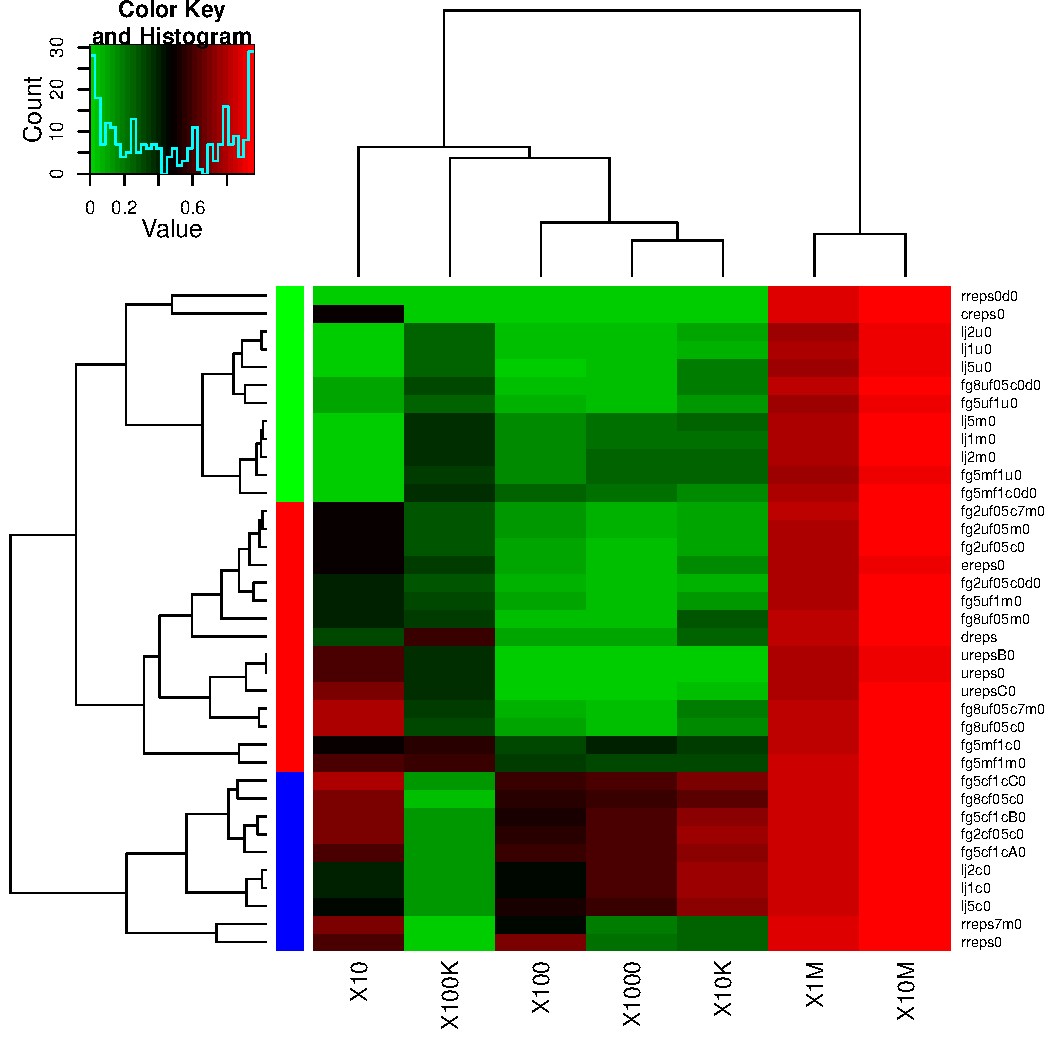
\includegraphics{figures/heatmap-srates-medians-0wk}
    \caption{Staying power clustering of all simulations started from scratch.}
    \label{figure:heatmap-srates-medians-0wk}
\end{center}
\end{figure}
Figure~\ref{figure:heatmap-srates-medians-1wk} shows staying power clustering of all of the basic simulations, seeded with one week of the {\itshape dreps} reality.



\begin{figure}
\begin{center}
    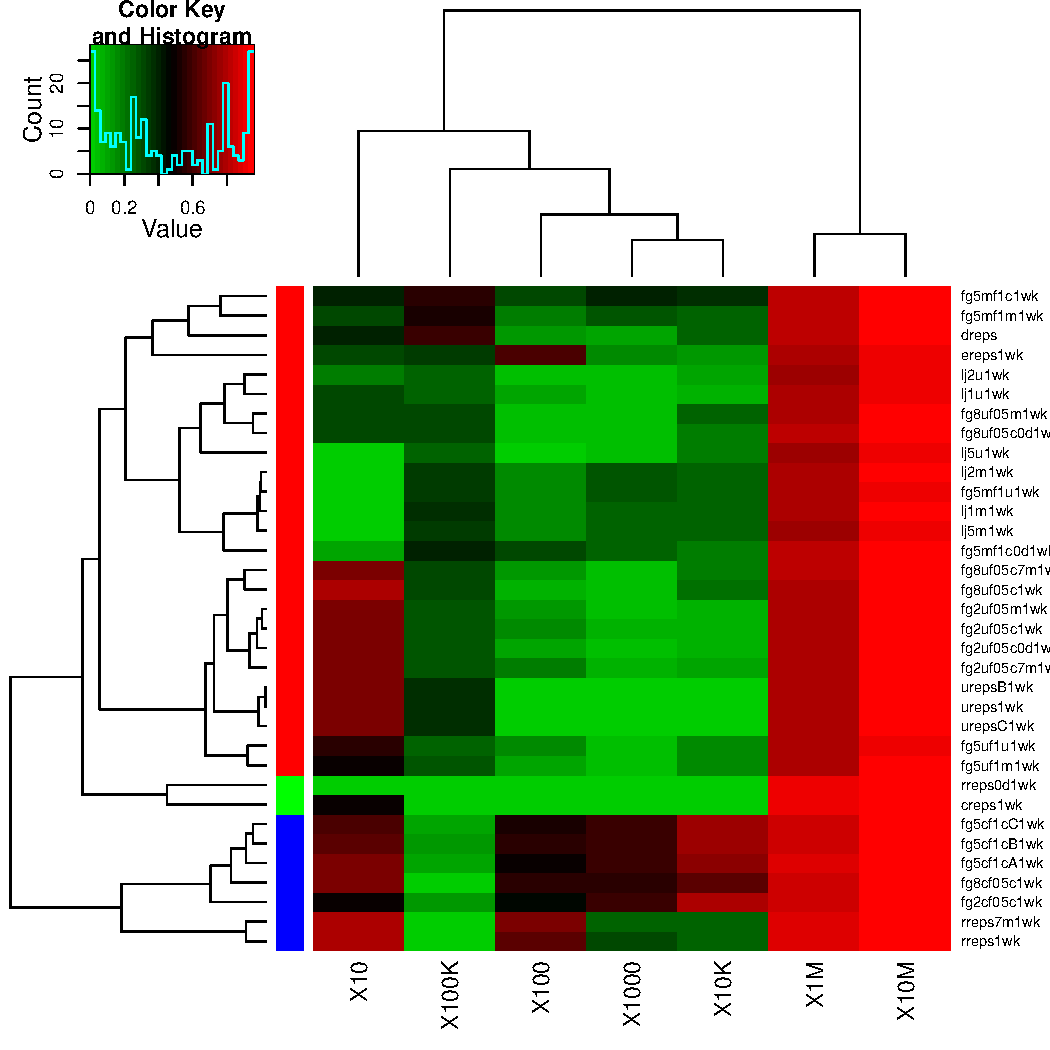
\includegraphics{figures/heatmap-srates-medians-1wk}
    \caption{Staying power clustering of all simulations seeded by 1 week of reality.}
    \label{figure:heatmap-srates-medians-1wk}
\end{center}
\end{figure}
Figure~\ref{figure:heatmap-srates-medians-2wk} shows staying power clustering of all of the basic simulations, seeded with two weeks of the {\itshape dreps} reality.



\begin{figure}
\begin{center}
    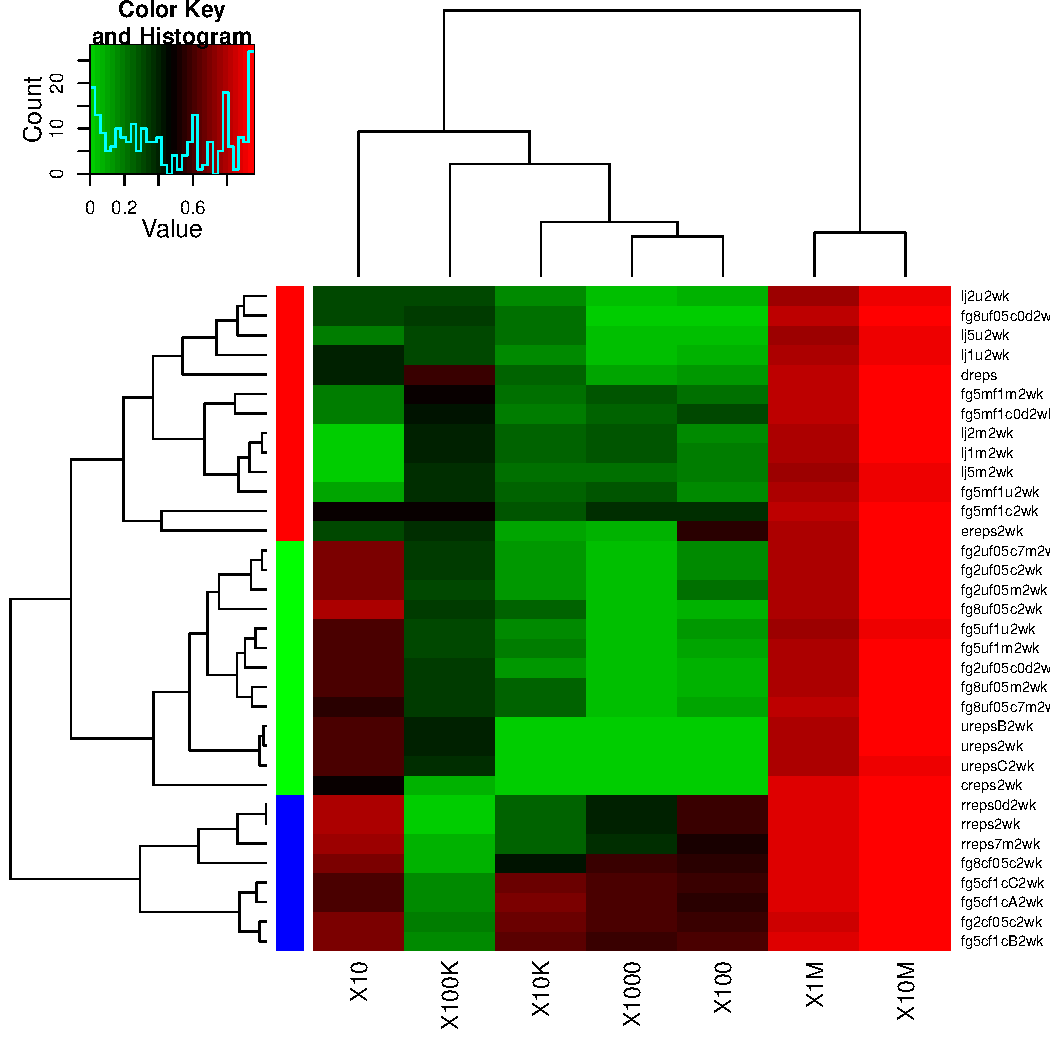
\includegraphics{figures/heatmap-srates-medians-2wk}
    \caption{Staying power clustering of all simulations seeded by 2 weeks of reality.}
    \label{figure:heatmap-srates-medians-2wk}
\end{center}
\end{figure}
Figures \ref{figure:heatmap-overx-dreps-medians-0wk},\ref{figure:heatmap-overx-dreps-medians-1wk},\ref{figure:heatmap-overx-dreps-medians-2wk},\ref{figure:heatmap-overx-dreps-medians-3wk} show the evolution of reality overlap as the amount of reality seeding increases.  


Global uniform strategies, also coupled with mentions or capital-based FOFs, are closer to reality when starting from scratch, then gradually yielding to global mentions and mentions-mentions-based ones, finally grouping with global capital and capital-capital-based simulations.  Smarter simulations achieve higher overlap with reality, especially when using our reciprocal social capital.


Figure~\ref{figure:heatmap-overx-dreps-medians-0wk} shows reality overlap clustering of all of the basic simulations, run from scratch without mixing any of the {\itshape dreps} reality itself.



\begin{figure}
\begin{center}
    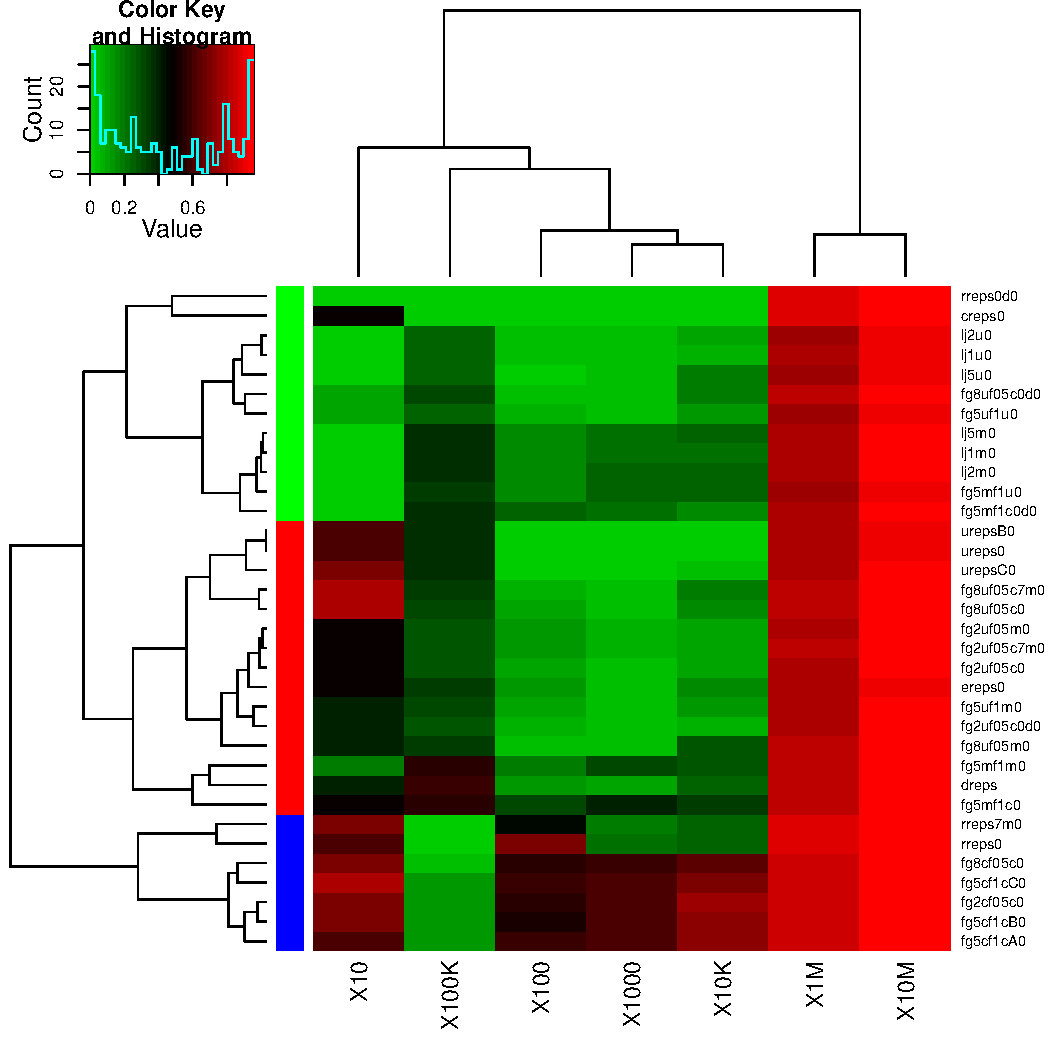
\includegraphics{figures/heatmap-overx-dreps-medians-0wk}
    \caption{Reality overlap clustering of all simulations started from scratch.}
    \label{figure:heatmap-overx-dreps-medians-0wk}
\end{center}
\end{figure}
Figure~\ref{figure:heatmap-overx-dreps-medians-1wk} shows reality overlap clustering of all of the basic simulations, run after mixing in one week of the {\itshape dreps} reality itself.



\begin{figure}
\begin{center}
    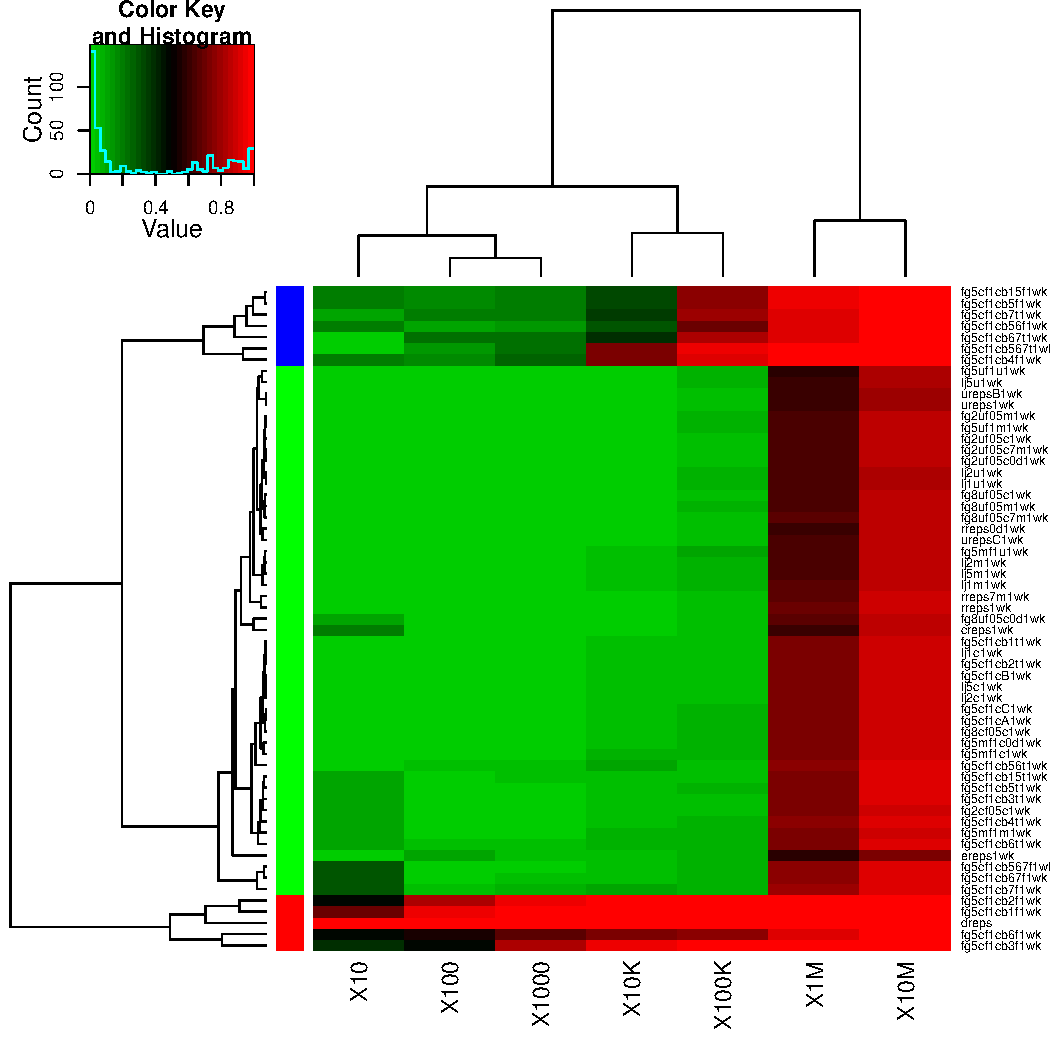
\includegraphics{figures/heatmap-overx-dreps-medians-1wk}
    \caption{Reality overlap clustering of all simulations seeded by 1 week of reality.}
    \label{figure:heatmap-overx-dreps-medians-1wk}
\end{center}
\end{figure}
Figure~\ref{figure:heatmap-overx-dreps-medians-2wk} shows reality overlap clustering of all of the basic simulations, run after mixing in two weeks of the {\itshape dreps} reality itself.



\begin{figure}
\begin{center}
    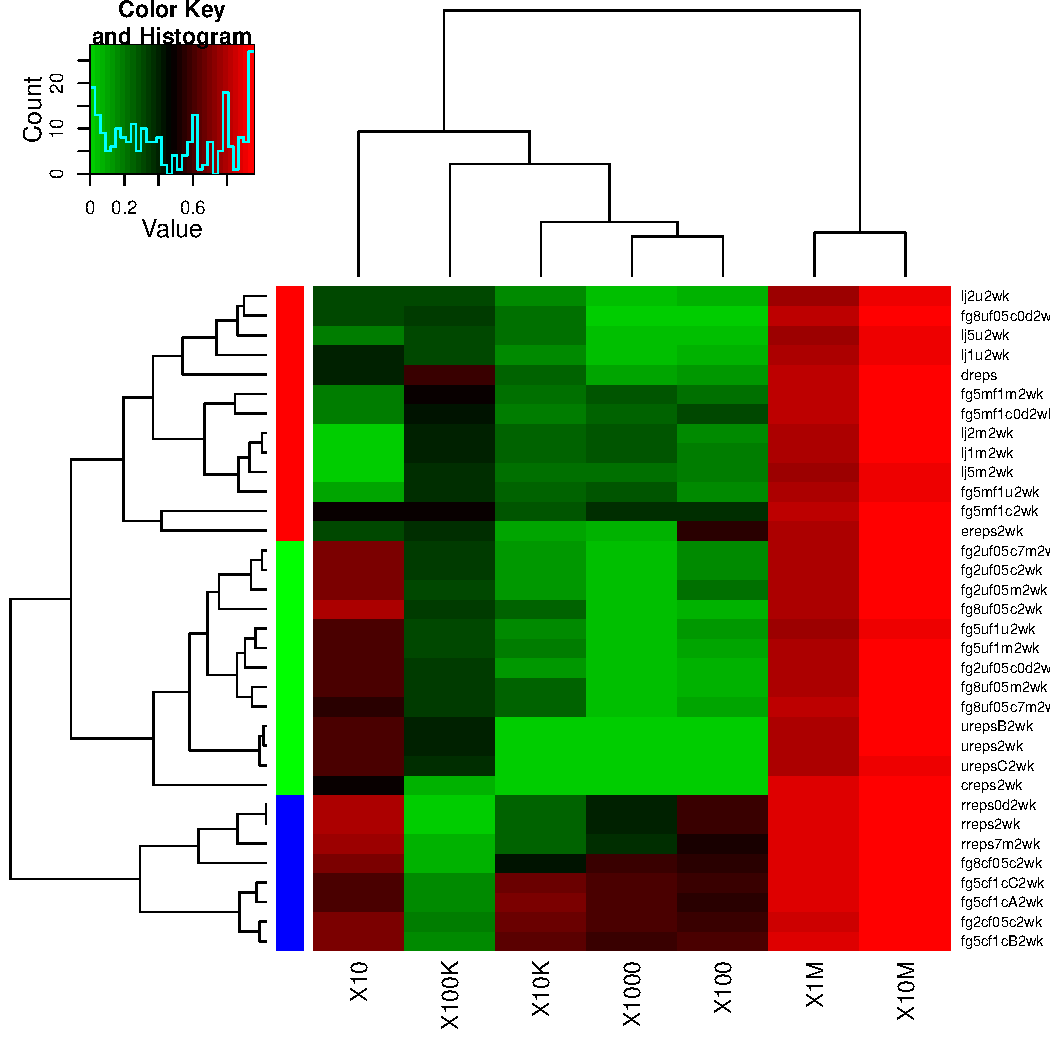
\includegraphics{figures/heatmap-overx-dreps-medians-2wk}
    \caption{Reality overlap clustering of all simulations seeded by 2 weeks of reality.}
    \label{figure:heatmap-overx-dreps-medians-2wk}
\end{center}
\end{figure}
Figure~\ref{figure:heatmap-overx-dreps-medians-3wk} shows reality overlap clustering of all of the basic simulations, run after mixing in three weeks of the {\itshape dreps} reality itself.



\begin{figure}
\begin{center}
    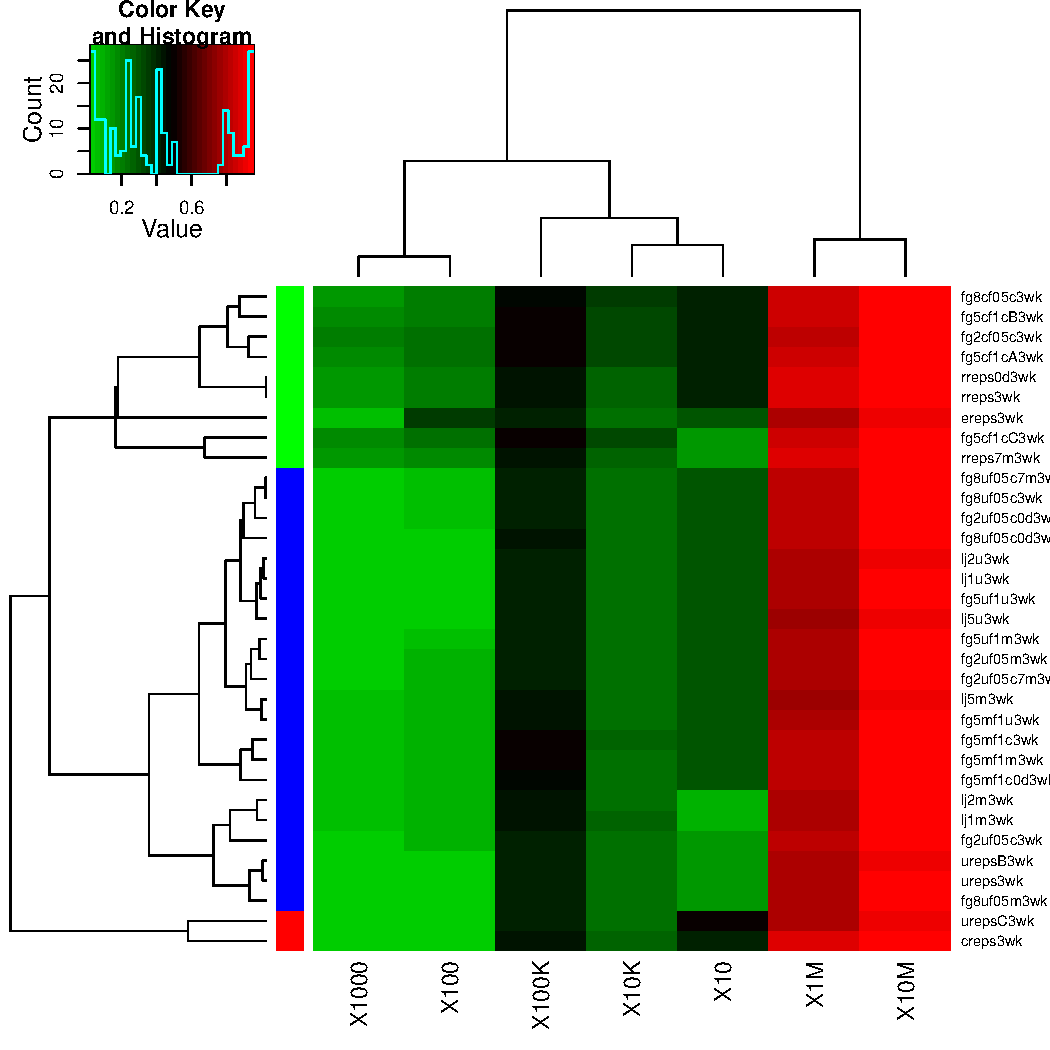
\includegraphics{figures/heatmap-overx-dreps-medians-3wk}
    \caption{Reality overlap clustering of all simulations seeded by 3 weeks of reality.}
    \label{figure:heatmap-overx-dreps-medians-3wk}
\end{center}
\end{figure}

\bibliography{/Users/alexyk/Documents/Thesis/bib/bibdesk/khrabrov-mindeconomy-thesis}

\appendixpage
\appendix
\chapter{A}
\counterwithin{table}{chapter}
\pagestyle{plain}
\newgeometry{hmargin=19mm,includefoot,top=1cm,bottom=15pt}
\section{Table Summaries}
\begin{table}
\centering
\minipage{0.50\textwidth}
\resizebox{\linewidth}{!}{
\begin{tabular}{|llccccccc|}
\toprule
\# & \emph{simulation} & 10 & 100 & 1K & 10K & 100K & 1M & 10M\\
\midrule
\input{ereps/srates/tex/n-ereps-srates-averages}
\bottomrule
\end{tabular}}
\caption{ereps-srates-averages}
\label{table:ereps-srates-averages}
\endminipage\hfill%
%
\minipage{0.50\textwidth}
\resizebox{\linewidth}{!}{
\begin{tabular}{|llccccccc|}
\toprule
\# & \emph{simulation} & 10 & 100 & 1K & 10K & 100K & 1M & 10M\\
\midrule
\input{ereps/srates/tex/n-ereps-srates-medians}
\bottomrule
\end{tabular}}
\caption{ereps-srates-medians}
\label{table:ereps-srates-medians}
\endminipage
\end{table}

\begin{table}
\centering
\minipage{0.50\textwidth}
\resizebox{\linewidth}{!}{
\begin{tabular}{|llccccccc|}
\toprule
\# & \emph{simulation} & 10 & 100 & 1K & 10K & 100K & 1M & 10M\\
\midrule
\input{lreps/srates/tex/n-lreps-srates-averages}
\bottomrule
\end{tabular}}
\caption{lreps-srates-averages}
\label{table:lreps-srates-averages}
\endminipage\hfill%
%
\minipage{0.50\textwidth}
\resizebox{\linewidth}{!}{
\begin{tabular}{|llccccccc|}
\toprule
\# & \emph{simulation} & 10 & 100 & 1K & 10K & 100K & 1M & 10M\\
\midrule
\input{lreps/srates/tex/n-lreps-srates-medians}
\bottomrule
\end{tabular}}
\caption{lreps-srates-medians}
\label{table:lreps-srates-medians}
\endminipage
\end{table}

\begin{table}
\centering
\minipage{0.50\textwidth}
\resizebox{\linewidth}{!}{
\begin{tabular}{|llccccccc|}
\toprule
\# & \emph{simulation} & 10 & 100 & 1K & 10K & 100K & 1M & 10M\\
\midrule
\input{ereps/overx/tex/n-ereps-overx-dreps-averages}
\bottomrule
\end{tabular}}
\caption{ereps-overx-dreps-averages}
\label{table:ereps-overx-dreps-averages}
\endminipage\hfill%
%
\minipage{0.50\textwidth}
\resizebox{\linewidth}{!}{
\begin{tabular}{|llccccccc|}
\toprule
\# & \emph{simulation} & 10 & 100 & 1K & 10K & 100K & 1M & 10M\\
\midrule
\input{ereps/overx/tex/n-ereps-overx-dreps-medians}
\bottomrule
\end{tabular}}
\caption{ereps-overx-dreps-medians}
\label{table:ereps-overx-dreps-medians}
\endminipage
\end{table}

\begin{table}
\centering
\minipage{0.50\textwidth}
\resizebox{\linewidth}{!}{
\begin{tabular}{|llccccccc|}
\toprule
\# & \emph{simulation} & 10 & 100 & 1K & 10K & 100K & 1M & 10M\\
\midrule
\input{lreps/overx/tex/n-lreps-overx-dreps-averages}
\bottomrule
\end{tabular}}
\caption{lreps-overx-dreps-averages}
\label{table:lreps-overx-dreps-averages}
\endminipage\hfill%
%
\minipage{0.50\textwidth}
\resizebox{\linewidth}{!}{
\begin{tabular}{|llccccccc|}
\toprule
\# & \emph{simulation} & 10 & 100 & 1K & 10K & 100K & 1M & 10M\\
\midrule
\input{lreps/overx/tex/n-lreps-overx-dreps-medians}
\bottomrule
\end{tabular}}
\caption{lreps-overx-dreps-medians}
\label{table:lreps-overx-dreps-medians}
\endminipage
\end{table}

\begin{table}
\centering
\minipage{0.50\textwidth}
\resizebox{\linewidth}{!}{
\begin{tabular}{|llccccccc|}
\toprule
\# & \emph{simulation} & 10 & 100 & 1K & 10K & 100K & 1M & 10M\\
\midrule
\input{ereps/overx/tex/n-ereps-overx-ereps-averages}
\bottomrule
\end{tabular}}
\caption{ereps-overx-ereps-averages}
\label{table:ereps-overx-ereps-averages}
\endminipage\hfill%
%
\minipage{0.50\textwidth}
\resizebox{\linewidth}{!}{
\begin{tabular}{|llccccccc|}
\toprule
\# & \emph{simulation} & 10 & 100 & 1K & 10K & 100K & 1M & 10M\\
\midrule
\input{ereps/overx/tex/n-ereps-overx-ereps-medians}
\bottomrule
\end{tabular}}
\caption{ereps-overx-ereps-medians}
\label{table:ereps-overx-ereps-medians}
\endminipage
\end{table}

\begin{table}
\centering
\minipage{0.50\textwidth}
\resizebox{\linewidth}{!}{
\begin{tabular}{|llccccccc|}
\toprule
\# & \emph{simulation} & 10 & 100 & 1K & 10K & 100K & 1M & 10M\\
\midrule
\input{lreps/overx/tex/n-lreps-overx-lreps-averages}
\bottomrule
\end{tabular}}
\caption{lreps-overx-lreps-averages}
\label{table:lreps-overx-lreps-averages}
\endminipage\hfill%
%
\minipage{0.50\textwidth}
\resizebox{\linewidth}{!}{
\begin{tabular}{|llccccccc|}
\toprule
\# & \emph{simulation} & 10 & 100 & 1K & 10K & 100K & 1M & 10M\\
\midrule
\input{lreps/overx/tex/n-lreps-overx-lreps-medians}
\bottomrule
\end{tabular}}
\caption{lreps-overx-lreps-medians}
\label{table:lreps-overx-lreps-medians}
\endminipage
\end{table}

\begin{table}
\centering
\minipage{0.50\textwidth}
\resizebox{\linewidth}{!}{
\begin{tabular}{|llccccccc|}
\toprule
\# & \emph{simulation} & 10 & 100 & 1K & 10K & 100K & 1M & 10M\\
\midrule
\input{freps/srates/tex/n-freps-srates-averages}
\bottomrule
\end{tabular}}
\caption{freps-srates-averages}
\label{table:freps-srates-averages}
\endminipage\hfill%
%
\minipage{0.50\textwidth}
\resizebox{\linewidth}{!}{
\begin{tabular}{|llccccccc|}
\toprule
\# & \emph{simulation} & 10 & 100 & 1K & 10K & 100K & 1M & 10M\\
\midrule
\input{freps/srates/tex/n-freps-srates-medians}
\bottomrule
\end{tabular}}
\caption{freps-srates-medians}
\label{table:freps-srates-medians}
\endminipage
\end{table}

\begin{table}
\centering
\minipage{0.50\textwidth}
\resizebox{\linewidth}{!}{
\begin{tabular}{|llccccccc|}
\toprule
\# & \emph{simulation} & 10 & 100 & 1K & 10K & 100K & 1M & 10M\\
\midrule
\input{freps/overx/tex/n-freps-overx-dreps-averages}
\bottomrule
\end{tabular}}
\caption{freps-overx-dreps-averages}
\label{table:freps-overx-dreps-averages}
\endminipage\hfill%
%
\minipage{0.50\textwidth}
\resizebox{\linewidth}{!}{
\begin{tabular}{|llccccccc|}
\toprule
\# & \emph{simulation} & 10 & 100 & 1K & 10K & 100K & 1M & 10M\\
\midrule
\input{freps/overx/tex/n-freps-overx-dreps-medians}
\bottomrule
\end{tabular}}
\caption{freps-overx-dreps-medians}
\label{table:freps-overx-dreps-medians}
\endminipage
\end{table}

\begin{table}
\centering
\minipage{0.50\textwidth}
\resizebox{\linewidth}{!}{
\begin{tabular}{|llccccccc|}
\toprule
\# & \emph{simulation} & 10 & 100 & 1K & 10K & 100K & 1M & 10M\\
\midrule
\input{freps/overx/tex/n-freps-overx-freps-averages}
\bottomrule
\end{tabular}}
\caption{freps-overx-freps-averages}
\label{table:freps-overx-freps-averages}
\endminipage\hfill%
%
\minipage{0.50\textwidth}
\resizebox{\linewidth}{!}{
\begin{tabular}{|llccccccc|}
\toprule
\# & \emph{simulation} & 10 & 100 & 1K & 10K & 100K & 1M & 10M\\
\midrule
\input{freps/overx/tex/n-freps-overx-freps-medians}
\bottomrule
\end{tabular}}
\caption{freps-overx-freps-medians}
\label{table:freps-overx-freps-medians}
\endminipage
\end{table}

\begin{table}
\centering
\minipage{0.50\textwidth}
\resizebox{\linewidth}{!}{
\begin{tabular}{|llccccccc|}
\toprule
\# & \emph{simulation} & 10 & 100 & 1K & 10K & 100K & 1M & 10M\\
\midrule
\input{ureps-deux/srates/tex/n-ureps-deux-srates-averages}
\bottomrule
\end{tabular}}
\caption{ureps-deux-srates-averages}
\label{table:ureps-deux-srates-averages}
\endminipage\hfill%
%
\minipage{0.50\textwidth}
\resizebox{\linewidth}{!}{
\begin{tabular}{|llccccccc|}
\toprule
\# & \emph{simulation} & 10 & 100 & 1K & 10K & 100K & 1M & 10M\\
\midrule
\input{ureps-deux/srates/tex/n-ureps-deux-srates-medians}
\bottomrule
\end{tabular}}
\caption{ureps-deux-srates-medians}
\label{table:ureps-deux-srates-medians}
\endminipage
\end{table}

\begin{table}
\centering
\minipage{0.50\textwidth}
\resizebox{\linewidth}{!}{
\begin{tabular}{|llccccccc|}
\toprule
\# & \emph{simulation} & 10 & 100 & 1K & 10K & 100K & 1M & 10M\\
\midrule
\input{ureps-deux/overx/tex/n-ureps-deux-overx-dreps-averages}
\bottomrule
\end{tabular}}
\caption{ureps-deux-overx-dreps-averages}
\label{table:ureps-deux-overx-dreps-averages}
\endminipage\hfill%
%
\minipage{0.50\textwidth}
\resizebox{\linewidth}{!}{
\begin{tabular}{|llccccccc|}
\toprule
\# & \emph{simulation} & 10 & 100 & 1K & 10K & 100K & 1M & 10M\\
\midrule
\input{ureps-deux/overx/tex/n-ureps-deux-overx-dreps-medians}
\bottomrule
\end{tabular}}
\caption{ureps-deux-overx-dreps-medians}
\label{table:ureps-deux-overx-dreps-medians}
\endminipage
\end{table}

\begin{table}
\centering
\minipage{0.50\textwidth}
\resizebox{\linewidth}{!}{
\begin{tabular}{|llccccccc|}
\toprule
\# & \emph{simulation} & 10 & 100 & 1K & 10K & 100K & 1M & 10M\\
\midrule
\input{ureps-deux/overx/tex/n-ureps-deux-overx-ureps-averages}
\bottomrule
\end{tabular}}
\caption{ureps-deux-overx-ureps-averages}
\label{table:ureps-deux-overx-ureps-averages}
\endminipage\hfill%
%
\minipage{0.50\textwidth}
\resizebox{\linewidth}{!}{
\begin{tabular}{|llccccccc|}
\toprule
\# & \emph{simulation} & 10 & 100 & 1K & 10K & 100K & 1M & 10M\\
\midrule
\input{ureps-deux/overx/tex/n-ureps-deux-overx-ureps-medians}
\bottomrule
\end{tabular}}
\caption{ureps-deux-overx-ureps-medians}
\label{table:ureps-deux-overx-ureps-medians}
\endminipage
\end{table}

\begin{table}
\centering
\minipage{0.50\textwidth}
\resizebox{\linewidth}{!}{
\begin{tabular}{|llccccccc|}
\toprule
\# & \emph{simulation} & 10 & 100 & 1K & 10K & 100K & 1M & 10M\\
\midrule
\input{freps-deux/srates/tex/n-freps-deux-srates-averages}
\bottomrule
\end{tabular}}
\caption{freps-deux-srates-averages}
\label{table:freps-deux-srates-averages}
\endminipage\hfill%
%
\minipage{0.50\textwidth}
\resizebox{\linewidth}{!}{
\begin{tabular}{|llccccccc|}
\toprule
\# & \emph{simulation} & 10 & 100 & 1K & 10K & 100K & 1M & 10M\\
\midrule
\input{freps-deux/srates/tex/n-freps-deux-srates-medians}
\bottomrule
\end{tabular}}
\caption{freps-deux-srates-medians}
\label{table:freps-deux-srates-medians}
\endminipage
\end{table}

\begin{table}
\centering
\minipage{0.50\textwidth}
\resizebox{\linewidth}{!}{
\begin{tabular}{|llccccccc|}
\toprule
\# & \emph{simulation} & 10 & 100 & 1K & 10K & 100K & 1M & 10M\\
\midrule
\input{freps-deux/overx/tex/n-freps-deux-overx-dreps-averages}
\bottomrule
\end{tabular}}
\caption{freps-deux-overx-dreps-averages}
\label{table:freps-deux-overx-dreps-averages}
\endminipage\hfill%
%
\minipage{0.50\textwidth}
\resizebox{\linewidth}{!}{
\begin{tabular}{|llccccccc|}
\toprule
\# & \emph{simulation} & 10 & 100 & 1K & 10K & 100K & 1M & 10M\\
\midrule
\input{freps-deux/overx/tex/n-freps-deux-overx-dreps-medians}
\bottomrule
\end{tabular}}
\caption{freps-deux-overx-dreps-medians}
\label{table:freps-deux-overx-dreps-medians}
\endminipage
\end{table}

\begin{table}
\centering
\minipage{0.50\textwidth}
\resizebox{\linewidth}{!}{
\begin{tabular}{|llccccccc|}
\toprule
\# & \emph{simulation} & 10 & 100 & 1K & 10K & 100K & 1M & 10M\\
\midrule
\input{freps-deux/overx/tex/n-freps-deux-overx-freps-averages}
\bottomrule
\end{tabular}}
\caption{freps-deux-overx-freps-averages}
\label{table:freps-deux-overx-freps-averages}
\endminipage\hfill%
%
\minipage{0.50\textwidth}
\resizebox{\linewidth}{!}{
\begin{tabular}{|llccccccc|}
\toprule
\# & \emph{simulation} & 10 & 100 & 1K & 10K & 100K & 1M & 10M\\
\midrule
\input{freps-deux/overx/tex/n-freps-deux-overx-freps-medians}
\bottomrule
\end{tabular}}
\caption{freps-deux-overx-freps-medians}
\label{table:freps-deux-overx-freps-medians}
\endminipage
\end{table}

%\input{ereps/srates/tex/dir-srates-ereps}
\input{lreps/srates/tex/dir-srates-lreps}
\input{ereps/overx/tex/dir-ereps-overx-dreps}
\input{lreps/overx/tex/dir-lreps-overx-dreps}
\input{ereps/overx/tex/dir-ereps-overx-ereps}
\input{lreps/overx/tex/dir-lreps-overx-lreps}
%\input{freps/srates/tex/dir-srates-freps}
\input{freps/overx/tex/dir-freps-overx-dreps}
\input{freps/overx/tex/dir-freps-overx-freps}
%\input{ureps-deux/srates/tex/dir-srates-ureps-deux}
\input{ureps-deux/overx/tex/dir-ureps-deux-overx-dreps}
\input{ureps-deux/overx/tex/dir-ureps-deux-overx-ureps}
%\input{freps-deux/srates/tex/dir-srates-freps-deux}
\input{freps-deux/overx/tex/dir-freps-deux-overx-dreps}
\input{freps-deux/overx/tex/dir-freps-deux-overx-freps}
\section{Staying Rates}
\label{sec:tables-srates}
\subsection{ereps staying rates}
\label{sub:tables-ereps-srates}
\input{ereps/srates/tex/dir-srates-ereps}
\subsection{lreps staying rates}
\label{sub:tables-lreps-srates}
\input{lreps/srates/tex/dir-srates-lreps}
\subsection{freps-staying-rates}
\label{sub:tables-freps-srates}
\input{freps/srates/tex/dir-srates-freps}
\subsection{ureps-deux staying rates}
\label{sub:tables-ureps-deux-srates}
\input{ureps-deux/srates/tex/dir-srates-ureps-deux}
\subsection{freps-deux staying rates}
\label{sub:tables-freps-deux-srates}
\input{freps-deux/srates/tex/dir-srates-freps-deux}
\section{Overlap with Real Buckets -- Dreps}
\label{sec:tables-overx-dreps}
\subsection{ereps overlap with dreps}
\label{sub:tables-ereps-overx-dreps}
\input{ereps/overx/tex/dir-ereps-overx-dreps}
\subsection{lreps overlap with dreps}
\label{sub:tables-lreps-overx-dreps}
\input{lreps/overx/tex/dir-lreps-overx-dreps}
\subsection{freps overlap with dreps}
\label{sub:tables-freps-overx-dreps}
\input{freps/overx/tex/dir-freps-overx-dreps}
\subsection{ureps-deux overlap with dreps}
\label{sub:tables-ureps-deux-overx-dreps}
\input{ureps-deux/overx/tex/dir-ureps-deux-overx-dreps}
\subsection{freps-deux overlap with dreps}
\label{sub:tables-tables-freps-deux-overx-dreps}
\input{freps-deux/overx/tex/dir-freps-deux-overx-dreps}
\section{Overlap with Its Own Class, Week-shifted and Cross-Run}
\label{sec:tables-overx-self}
\subsection{ereps overlap with ereps}
\label{sub:tables-ereps-overx-ereps}
\input{ereps/overx/tex/dir-ereps-overx-ereps}
\subsection{lreps overlap with lreps}
\label{sub:tables-lreps-overx-lreps}
\input{lreps/overx/tex/dir-lreps-overx-lreps}
\subsection{freps overlap with freps}
\label{sub:tables-freps-overx-freps}
\input{freps/overx/tex/dir-freps-overx-freps}
\subsection{ureps-deux overlap with ureps and ureps-deux}
\label{sub:tables-ureps-deux-overx-ureps}
\input{ureps-deux/overx/tex/dir-ureps-deux-overx-ureps}
\subsection{freps-deux overlap with freps and freps-deux}
\label{sub:tables-freps-deux-overx-ereps}
\input{freps-deux/overx/tex/dir-freps-deux-overx-freps}
%
% Back Matter
%

\backmatter
%\appendixpage

%	Bibliography
\bibliographystyle{\mybibliostyle}
\bibliocommand

%	Glossary
\printglossary


%	Index
\printindex

\end{document}
